\hypertarget{contributions}{%
\section{Contributions}\label{contributions}}

This material is this chapter expands on work presented in

\autocite{hodsonOnedimensionalLongRangeFalikovKimball2021} \href{https://link.aps.org/doi/10.1103/PhysRevB.104.045116}{One-dimensional long-range Falikov-Kimball model: Thermal phase transition and disorder-free localization}, Hodson, T. and Willsher, J. and Knolle, J., Phys. Rev.~B, \textbf{104}, 4, 2021,

Johannes had the initial idea to use a long range Ising term to stablise order in a one dimension Falikov-Kimball model. Josef developed a proof of concept during a summer project at Imperial. The three of us brought the project to fruition.

\hypertarget{introduction}{%
\section{Introduction}\label{introduction}}

\hypertarget{localisation}{%
\subsection{Localisation}\label{localisation}}

The discovery of localisation in quantum systems surprising at the time given the seeming ubiquity of extended Bloch states. Later, when thermalisation in quantum systems gained interest, localisation phenomena again stood out as counterexamples to the eigenstate thermalisation hypothesis \autocite{abaninRecentProgressManybody2017,srednickiChaosQuantumThermalization1994}, allowing quantum systems to avoid to retain memory of their initial conditions in the face of thermal noise.

The simplest and first discovered kind is Anderson localisation, first studied in 1958 \textcite{andersonAbsenceDiffusionCertain1958} in the context of non-interacting fermions subject to a static or quenched disorder potential \(V_j\) drawn uniformly from the interval \([-W,W]\)

\[
H = -t\sum_{\langle jk \rangle} c^\daggerger_j c_k + \sum_j V_j c_j^\daggerger c_j
\]

this model exhibits exponentially localised eigenfunctions \(\psi(x) = f(x) e^{-x/\lambda}\) which cannot contribute to transport processes. Initially it was thought that in one dimensional disordered models, all states would be localised, however it was later shown that in the presence of correlated disorder, bands of extended states can exist \autocite{izrailevLocalizationMobilityEdge1999,croyAndersonLocalization1D2011,izrailevAnomalousLocalizationLowDimensional2012}.

Later localisation was found in interacting many-body systems with quenched disorder:

\[
H = -t\sum_{\langle jk \rangle} c^\daggerger_j c_k + \sum_j V_j c_j^\daggerger c_j + U\sum_{jk} n_j n_k
\]

where the number operators \(n_j = c^\dagger_j c_j\). Here, in contrast to the Anderson model, localisation phenomena can be proven robust to weak perturbations of the Hamiltonian. This is called many-body localisation (MBL) \textcite{imbrieManyBodyLocalizationQuantum2016}.

Both MBL and Anderson localisation depend crucially on the presence of quenched disorder. This has led to ongoing interest in the possibility of disorder-free localisation, in which the disorder necessary to generate localisation is generated entirely from the dynamics of the model. This contracts with typical models of disordered systems in which disorder is explicielty introduced into the Hamilton or the initial state.

The concept of disorder-free localisation was first proposed in the context of Helium mixtures \textcite{kagan1984localization} and then extended to heavy-light mixtures in which multiple species with large mass ratios interact. The idea is that the heavier particles act as an effective disorder potential for the lighter ones, inducing localisation. Two such models \autocite{yaoQuasiManyBodyLocalizationTranslationInvariant2016,schiulazDynamicsManybodyLocalized2015} instead find that the models thermalise exponentially slowly in system size, which Ref. \textcite{yaoQuasiManyBodyLocalizationTranslationInvariant2016} dubs Quasi-MBL.

True disorder-free localisation does occur in exactly solveable models with extensively many conserved quantities \textcite{smithDisorderFreeLocalization2017}. As conserved quantites have no time dynamics this can be thought of as taking the separation of timescales to the infinite limit.

\hypertarget{the-falikov-kimball-model}{%
\subsubsection{The Falikov Kimball Model}\label{the-falikov-kimball-model}}

In the Falikov Kimball (FK) model spinless fermions \(c_{i\uparrow}\) are coupled via a repulsive on-site interaction to a classical degree of freedom \(n_{i\downarrow}\).

\[\begin{aligned}
H &= -t \sum_{<ij>} c^\daggerger_{i\uparrow}c_{j\uparrow} + U \sum_{i} (n_{i \uparrow} - 1/2)( n_{i\downarrow} - 1/2) \\
       & - \mu \sum_i \left( n_{i \uparrow} + n_{i \downarrow} \right) + \sum_{ij} V_{ij} (n_{i\downarrow} - 1/2)(n_{j\downarrow} - 1/2) 
\end{aligned}\] \textbf{replace with hamiltonian from the paper}

This notation emphasises that this can also be thought of as an asymmetric Hubbard model in which the spin down electrons cannot hop and are subject to an additional long range potential. However, to avoid the confusion of talking about two distinct species of spinless electrons we will use a different interpretation and refer to the classical degrees of freedom as the ``ionic sector'' and the quantum degrees of freedom as the ``electronic sector''. The final term that induces interactions between the classical particles has been added by us to stabilise the formation of an ordered phase in 1D. The classical variables commute with the Hamiltonian \([H, n_{i\downarrow}] = 0\) so like the lattice gauge model in Ref \textcite{smithDisorderFreeLocalization2017}\} the FK model has extensively many conserved quantities which can act as an effective disorder potential for the electronic sector.

Due to Pauli exclusion, the maximum filling occurs when one of each species occupies each lattice site such that \(\sum_i (n_{i\downarrow} + n_{i\uparrow} )/ N = 2\). Here we focus on the half filled case which also displays particle-hole symmetry (see later).

\hypertarget{falikov-kimball-and-hubbard-models}{%
\subsection{Falikov Kimball and Hubbard models}\label{falikov-kimball-and-hubbard-models}}

We will first introduce the standard Hubbard and Falikov-Kimball (FK) models then look at some of their properties. We'll then cover why the Falikov-Kimball model represents an interesting system in which to study disorder free localisation.

\hypertarget{hubbard-model}{%
\subsubsection{Hubbard model}\label{hubbard-model}}

The Hubbard model gives a very simple setting in which to study interacting, itinerant electrons. It is a tight binding model of spin half electrons with finite bandwidth \(t\) and a repulsive on-site interaction \(U > 0\).

\[
    H = -\sum_{<ij>,\sigma} t_{\sigma} c^\dagger_{i\sigma}c_{j\sigma} + U \sum_{i} (n_{i \uparrow} - 1/2)( n_{i\downarrow} - 1/2) - \mu \sum_i \left( n_{i \uparrow} + n_{i \downarrow} \right)
\]

in standard notation. The standard Hubbard model corresponds to the case \(t_{\uparrow} = t_{\downarrow}\). Here we have used the particle-hole symmetric version of the interaction term, which is more often given as \(n_{i \uparrow} n_{i\downarrow}\). The difference just amounts to a redefinition of the chemical potential.

Hubbard originally used the model at half filling \(\mu = 0\) to explain the Mott metal-insulator (MI) transition, however it has seen applications to high-temperature superconductivity and become target for cold-atom optical trap experiments. \textcite{HubbardModelHalf2013}, greiner\_quantum\_2002, jordens\_mott\_2008\}. While simple, only a few analytic results exist, namely the Bethe ansatz \textcite{liebAbsenceMottTransition1968}\} which proves the absence of even a zero temperature phase transition in the 1D model and Nagaoka's theorem \textcite{nagaokaFerromagnetismNarrowAlmost1966}\} which proves that the three dimensional model has a ferromagnetic ground state in the vicinity of half filling.

\hypertarget{falikov-kimball-model}{%
\subsubsection{Falikov-Kimball model}\label{falikov-kimball-model}}

\begin{figure}
  \centering
    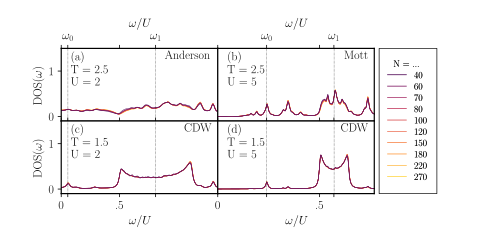
\includegraphics[width=\textwidth]{figs/DOS}
  \caption{Density of states for the Anderson model with (a) no potential, (b) a charge density wave (CDW) potential $\vec{h} = (0,1,0,1...)$, (c) a disordered CDW potential each site has an uncorrelated $2\%$ chance of deviating from the CDW background. Hopping and potential terms both have unit magnitude.}
  \label{fig:fk_dos}
\end{figure}

The Falikov-Kimball model corresponds to the case \(t_{\downarrow} = 0\). It can be interpreted as two coupled spinless electron bands with infinite mass ratio. An itinerant light species with creation operator \(c^\dagger_{i\uparrow}\) coupled to an infinitely heavy, immobile species with density operator \(n_{i\downarrow}\). These are often called c and f electrons or electrons and ions. The model was first introduced by Hubbard in 1963 as a model of interacting localised and de-localised electron bands and gained its name from Falikov and Kimball's use of it to study the MI transition in rare-earth materials \textcite{hubbardj.ElectronCorrelationsNarrow1963}, falicov\_simple\_1969\}.

Here we will use refer to the light spinless species as \texttt{electrons\textquotesingle{}\ with\ creation\ operator\ \$c\^{}\textbackslash{}dagger\_\{i\}\$\ and\ the\ heavy\ species\ as}ions' with density operator \(n_i\). When the the density operator of the electrons is needed I'll always use \(c^\dagger_{i}c_{i}\). We also set \(t = 1\).

\[
    H_{\mathrm{FK}} = -\sum_{<ij>} c^\dagger_{i}c_{j} + U \sum_{i} (c^\dagger_{i}c_{i} - 1/2)( n_i - 1/2) - \mu \sum_i \left(c^\dagger_{i}c_{i} + n_{i}\right)
\] \% \#\#\# Particle-Hole Symmetry The Hubbard and FK models on a bipartite lattice have particle-hole (PH) symmetry \(P^\dagger H P = - H\), accordingly they have symmetric energy spectra. The associated symmetry operator \(P\) exchanges creation and annihilation operators along with a sign change between the two sublattices.

\[ d^\dagger_{i\sigma} = (-1)^i c_{i\sigma}\] \% The entirely filled state \(\ket{\Omega} = \sum_{j\rho} c^\dagger_{j\rho} \ket{0}\) becomes the new vacuum state: \[d_{i\sigma} \ket{\Omega} = (-1)^i c^\dagger_{i\sigma} \sum_{j\rho} c^\dagger_{j\rho} \ket{0} = 0\] \% The number operator \(n_{i\sigma} = 0,1\) counts holes rather than particles: \[ d^\dagger_{i\sigma} d_{i \sigma} = c_{i\sigma} c^\dagger_{i\sigma} = 1 - c^\dagger_{i\sigma} c_{i\sigma}\] \% With the last equality following from the fermionic commutation relations. In the case of nearest neighbour hopping on a bipartite lattice this transformation also leaves the hopping term unchanged: \[ d^\dagger_{i\sigma} d_{j \sigma} = (-1)^{i+j} c_{i\sigma} c^\dagger_{j\sigma} = c^\dagger_{i\sigma} c_{j\sigma} \] \% Since when \(i\) and \(j\) label sites on separate sublattices, \((-1)^{i-j} = -1\) and this is absorbed into rearranging the operators via their anti-commutator.

Defining the particle density \(\rho\) as the number of fermions per site: \[
    \rho = \frac{1}{N} \sum_i \left( n_{i \uparrow} + n_{i \downarrow} \right)
\] \% The PH symmetry maps the Hamiltonian to itself with the sign of the chemical potential reversed and the density is inverted about half filling: \[ \text{PH} : H(t, U, \mu) \rightarrow H(t, U, -\mu) \] \[ \rho \rightarrow 2 - \rho \] \% The Hamiltonian is symmetric under PH at \(\mu = 0\) and so must all the observables, hence half filling \(\rho = 1\) occurs here. This symmetry and known observable acts as a useful test for the numerical calculations.

\hypertarget{thermodynamics-of-the-fk-model}{%
\subsubsection{Thermodynamics of the FK model}\label{thermodynamics-of-the-fk-model}}

\textbackslash begin\{figure\} \centering 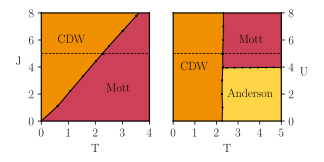
\includegraphics[width=0.8\textwidth]{figs/phase_diagram}

\caption{Phases of the 2D Falikov Kimball Model, showing the ordered charge density wave phase at low temperatures and the interaction mediated transition between Anderson localisation and Mott insulating phases in the disordered phase. @andersonAbsenceDiffusionCertain1958}

\} \label{fig:FK_phase_diagram} \textbackslash end\{figure\}

At half filling and in dimensions greater than one, the FK model exhibits a phase transition at some \(U\) dependent critical temperature \(T_c(U)\) to a low temperature charge density wave state in which the ions occupy one of the two sublattices A and B \textcite{maskaThermodynamicsTwodimensionalFalicovKimball2006}\}. The order parameter is the square of the staggered magnetisation: \[
M = \sum_{i \in A} n_i - \sum_{i \in B} n_i
\] \% In the disordered phase Ref. \textcite{andersonAbsenceDiffusionCertain1958}\} identifies an interplay between Anderson localisation at weak interaction and a Mott insulator phase in the strongly interacting regime.

In the one dimensional FK model, however, Peierls' argument \textcite{peierlsIsingModelFerromagnetism1936}, kennedyItinerantElectronModel1986\} and the Bethe ansatz \textcite{liebAbsenceMottTransition1968}\} make it clear that there is no ordered CDW phase. Peierls' argument is that one should consider the difference in free energy \(\Delta F = \Delta E - T\Delta S\) between an ordered state and a state with single domain wall in the order parameter. In the Ising model this would be having the spins pointing up in one part of the model and down in the other, for a CDW phase it means having the ions occupy the A sublattice in one part and the B sublattice in the other.

Short range interactions will produce a constant energy penalty for such a domain wall that does not scale with system size while in 1D there are \(L\) such states so the domain wall is associated with entropy \(S \propto \ln L\) which dominates in the thermodynamic limit. The slow logarithmic scaling suggests we should be wary of finite size scaling effects.

One dimensional systems are more amenable to numerical and experimental study so we add long range staggered interactions to bring back the ordered phase:

\[ H_{\textrm{int}} = 4J \sum_{ij} \frac{(-1)^{|i-j|}}{ |i - j|^{\alpha} } (n_i - 1/2) (n_j - 1/2) = J \sum_{ij} |i - j|^{-\alpha} \tau_i \tau_j\] \% at half-filling the modified Hamiltonian is then: \[
    H_{\mathrm{FK}}^* &= -\sum_{<ij>} c^\dagger_{i}c_{j} + U \sum_{i} (c^\dagger_{i}c_{i} - 1/2)( n_i - 1/2) \\
    &+ 4J \sum_{ij} \frac{(-1)^{|i-j|}}{ |i - j|^{\alpha} } (n_i - 1/2) (n_j - 1/2)  \\
    &= -\sum_{<ij>} c^\dagger_{i}c_{j} + 2U \sum_{i} (-1)^i (c^\dagger_{i}c_{i} - 1/2)\tau_i + J \sum_{ij} |i - j|^{-\alpha} \tau_i \tau_j  \\
\] \% The form of this interaction comes from interpreting the f-electrons as a classical Ising chain using a staggered mapping \(\tau_i = (-1)^i (2n_i^ f - 1)\) so that ferromagnetic order in the \(\tau_i\) variables corresponds to a CDW state in the \(n_i^f\) variables. It also preserves the particle hole symmetry because for the ions the PH transformation corresponds to \(n_i \rightarrow 1 - n_i\). When \(U = 0\) the model decouples into a long ranged Ising model and free fermions.

\subsubsection{Long Ranged Ising model}

Our extension to the FK model could now be though of as spinless fermions coupled to a long range Ising (LRI) model. The LRI model has been extensively studied and its behaviour may be bear relation to the behaviour of our modified FK model.

\[H_{\mathrm{LRI}} = \sum_{ij} J(\abs{i-j}) \tau_i \tau_j = J \sum_{i\neq j} |i - j|^{-\alpha} \tau_i \tau_j\] \% Rigorous renormalisation group arguments show that the LRI model has an ordered phase in 1D for \$1 \textless{} \alpha \textless{} 2 \$ \textcite{dysonExistencePhasetransitionOnedimensional1969}\}. Peierls' argument can be extended \textcite{thoulessLongRangeOrderOneDimensional1969}\} to provide intuition for why this is the case. Again considering the energy difference between the ordered state \(\ket{\ldots\uparrow\uparrow\uparrow\uparrow\ldots}\) and a domain wall state \(\ket{\ldots\uparrow\uparrow\downarrow\downarrow\ldots}\). In the case of the LRI model, careful counting shows that this energy penalty is: \[\Delta E \propto \sum_{n=1}^{\infty} n J(n)\] \% because each interaction between spins separated across the domain by a bond length \(n\) can be drawn between \(n\) equivalent pairs of sites. Ruelle proved rigorously for a very general class of 1D systems, that if \(\Delta E\) or its many-body generalisation converges in the thermodynamic limit then the free energy is analytic \textcite{ruelleStatisticalMechanicsOnedimensional1968}\}. This rules out a finite order phase transition, though not one of the Kosterlitz-Thouless type. Dyson also proves this though with a slightly different condition on \(J(n)\) \textcite{dysonExistencePhasetransitionOnedimensional1969}\}.

With a power law form for \(J(n)\), there are three cases to consider:

\begin{center}
    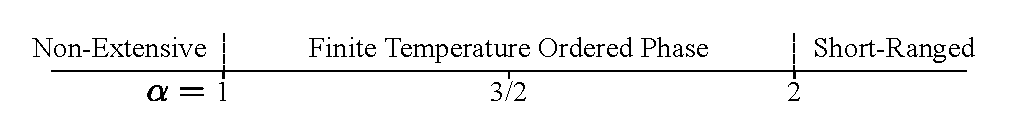
\includegraphics[width=\textwidth]{figs/alpha_diagram}
\end{center}

\begin{enumerate}
\def\labelenumi{\arabic{enumi}.}
\tightlist
\item
  \$ \alpha = 0\$ For infinite range interactions the Ising model is exactly solveable and mean field theory is exact \textcite{lipkinValidityManybodyApproximation1965}\}.
\item
  \$ \alpha \le 1\$ For slowly decaying interactions \(\sum_n J(n)\) does not converge so the Hamiltonian is non-extensive, a case which won't be further considered here.
\item
  \$ 1 \textless{} \alpha \textless{} 2 \$ A phase transition to an ordered state at a finite temperature.
\item
  \$ \alpha = 2 \$ The energy of domain walls diverges logarithmically, and this turns out to be a Kostelitz-Thouless transition \textcite{thoulessLongRangeOrderOneDimensional1969}\}.
\item
  \$ 2 \textless{} \alpha \$ For quickly decaying interactions, domain walls have a finite energy penalty, hence Peirels' argument holds and there is no phase transition.
\end{enumerate}

\hypertarget{thermodynamics}{%
\subsubsection{Thermodynamics}\label{thermodynamics}}

On bipartite lattices in dimensions 2 and above the FK model exhibits a finite temperature phase transition to an ordered charge density wave (CDW) phase \textcite{maskaThermodynamicsTwodimensionalFalicovKimball2006}. In this phase, the ions are confined to one of the two sublattices, breaking the \(\mathbb{Z}_2\) symmetry.

In 1D, however, Periel's argument \autocite{peierlsIsingModelFerromagnetism1936,kennedyItinerantElectronModel1986} states that domain walls only introduce a constant energy penalty into the free energy while bringing a entropic contribution logarithmic in system size. Hence the 1D model does not have a finite temperature phase transition. However 1D systems are much easier to study numerically and admit simpler realisations experimentally. We therefore introduce a long range coupling between the ions in order to stabilise a CDW phase in 1D. This leads to a disordered system that is gaped by the CDW background but with correlated fluctuations leading to a disorder-free correlation induced mobility edge in one dimension.

\hypertarget{markov-chain-monte-carlo}{%
\subsubsection{Markov Chain Monte Carlo}\label{markov-chain-monte-carlo}}

To evaluate thermodynamic averages we perform a classical Markov Chain Monte Carlo random walk over the space of ionic configurations, at each step diagonalising the effective electronic Hamiltonian \textcite{maskaThermodynamicsTwodimensionalFalicovKimball2006}\}. Using a binder-cumulant method \autocite{binderFiniteSizeScaling1981,musialMonteCarloSimulations2002}, we demonstrate the model has a finite temperature phase transition when the interaction is sufficiently long ranged. We then estimate the density of states and the inverse participation ratio as a function of energy to diagnose localisation properties. We show preliminary results that the in-gap states induced at finite temperature are localised while the states in the unperturbed bands remain extended, evidence for a mobility edge.

\begin{figure}
\hypertarget{fig:binder}{%
\centering
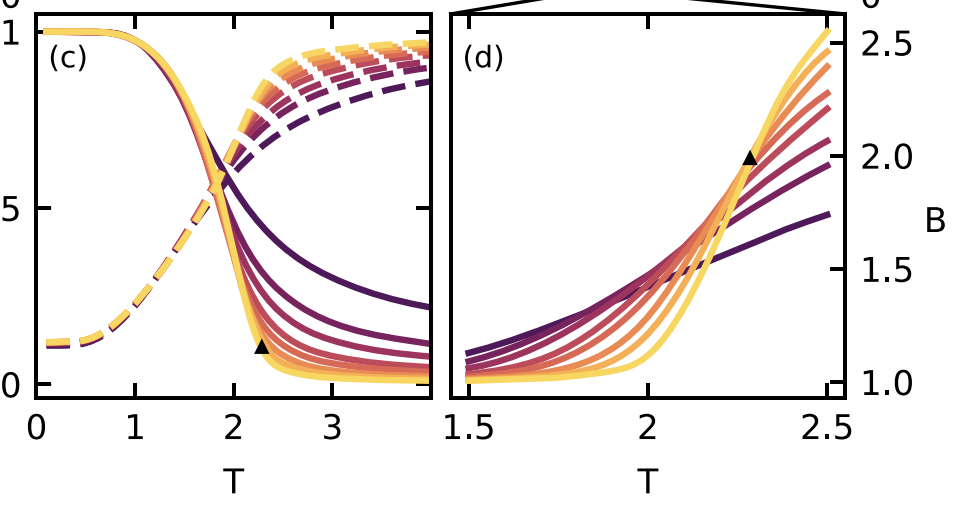
\includegraphics[width=1\textwidth,height=\textheight]{figure_code/fk_chapter/binder.png}
\caption{Hello I am the figure caption!}\label{fig:binder}
}
\end{figure}

Macro definitions in this cell \[
\newcommand{\expval}[1]{\langle #1 \rangle}
\newcommand{\ket}[1]{|#1\rangle}
\newcommand{\bra}[1]{\langle#1|}
\newcommand{\op}[2]{|#1\rangle \langle#2|}
\]

\[
\expval{O}, \op{\alpha}{\beta}, \ket{\psi}
\]

\hypertarget{localisation-1}{%
\subsection{Localisation}\label{localisation-1}}

\hypertarget{thermalisation}{%
\subsubsection{Thermalisation}\label{thermalisation}}

Isolated classical systems generally thermalise if they are large enough. Since classical dynamics is the limit of some underlying quantum dynamics, it seems reasonable to suggest that isolated quantum systems also thermalise in some related sense. However it is not immediately obvious what thermalisation should mean in a quantum setting where the presence of unitary time dynamics implies full information about a system's initial state is always preserved.

A potential solution lies in the eigenstate thermalisation hypothesis. It states that if a system thermalises, then we can isolate small patches of a larger system, trace everyhing else out, and get a thermal density matrix.

Following Ref. \textcite{abaninRecentProgressManybody2017}, consider the time evolution of a local operator \(\hat{O}\) \[ \expval{\hat{O}}{\psi(t)} = \sum_{\alpha \beta} C^*_\alpha C_\beta e^{i(E_\alpha - E_\beta)} O_{\alpha \beta}\]

Where \(C_\alpha\) are determined by the initial state and \(O_{\alpha \beta} = \expval{\alpha | \hat{O} | \beta}\) are the matrix elements of \(\hat{O}\) with respect to the energy eigenstates. Srednicki \textcite{srednickiChaosQuantumThermalization1994}\} introduced the ansatz that for local operators:

\[O_{\alpha \beta} = O(E)\delta_{\alpha\beta} + e^{-S(E)/2} f(E,\omega) R_{\alpha\beta}\]

with \(E = (E_\alpha + E_\beta)\), \(\omega = (E_\alpha - E_\beta)\) and \(R_{\alpha\beta}\) are sampled from some distribution with zero mean and unit variance. The first term asserts that the diagonal elements are given by the thermal expectation value \(O(E) = Tr[e^{-\beta \hat{H}} \hat{O}]/\mathcal{Z}\) with \(\beta\) an effective temperature defined by equating the energy to the expectation of the Hamiltonian at that temperature \(E = Tr[H e^{-\beta \hat{H}}/\mathcal{Z}]\).

The second term deals with thermodynamic fluctuations scaled by the entropy \(S(E) = -Tr(\rho \log \rho)\) where \(\rho = e^{-\beta \hat{H}}\) and \(\mathcal{Z} = Tr[e^{-\beta \hat{H}}]\).

With this ansatz the long time average of the observable becomes equal to the thermal expectations with fluctuations suppressed by the entropic term \(e^{-S(E)}\) and the rapidly varying phase factors \(e^{i(E_\alpha - E_\beta)}\). This statement of the ETH has verified for the quantum hard sphere model \textcite{srednickiChaosQuantumThermalization1994} and numerically for other models \autocite{khatamiFluctuationDissipationTheoremIsolated2013,dalessioQuantumChaosEigenstate2016}.

An alternate view on ETH is the statement that in thermalising systems individual eigenstates look thermal when viewed locally. Take a eigenstate \(|\alpha\rangle\) with energy \(E_\alpha\) and as before define an effective temperature with \(E_\alpha = Tr[H e^{-\beta \hat{H}}/\mathcal{Z}]\). This statement of the ETH says that if we partition the system into subsystems A and B with a limit taken as B becomes very large, B will act as a heat bath for A. Specifically the reduced density matrix \(\rho_A = Tr_B \op{\alpha}{\alpha}\) is equal to the thermal density matrix:

\[\rho_A = Tr_B |\alpha\rangle \langle \alpha| = \mathcal{Z}^{-1} Tr_B [e^{-\beta \hat{H}}] \]

Intuitively, for thermalisation to happen, the degrees of freedom must be sufficiently well coupled that energy transport occurs. This condition is broken by systems with localised states so a lack of thermalisation is often used as a diagnostic tool for localisation.

\hypertarget{anderson-localisation}{%
\subsubsection{Anderson Localisation}\label{anderson-localisation}}

Localisation was first studied by Anderson in 1958 \textcite{andersonAbsenceDiffusionCertain1958} in the context of non-interacting fermions subject to a static or quenched disorder potential \(V_j\) drawn uniformly from the interval \([-W,W]\):

\[
H = -t\sum_{\expval{jk}} c^\dagger_j c_k + \sum_j V_j c_j^\dagger c_j
\]

At sufficiently strong disorder the Anderson model exhibits exponentially localised eigenfunctions \(\psi(x) = f(x) e^{-x/\lambda}\) which cannot contribute to diffusive transport processes. Except in 1D where any disorder strength is sufficient. Intuitively this happens because hopping processes between nearby sites become off-resonant, hindering the hybridisation that would normally lead to extended Bloch states \textcite{kramerLocalizationTheoryExperiment1993}.

In one and two dimensions, all the states in the Anderson model are localised. In three dimensions there are mobility edges. Mobility edges are critical energies in the spectrum which separate delocalised states in a band from localised states which form a band tail \textcite{abaninRecentProgressManybody2017}\}. An argument due to Lifshitz shows that the density of state of the band tail should decay exponentially and localised and extended stats cannot co-exist at the same energy as they would hybridise into extended states \textcite{kramerLocalizationTheoryExperiment1993}\}.

It was thought that mobility edges could not exist in 1D because all the states localised in the presence of any amount of disorder. This is true for uncorrelated potentials \textcite{goldshteinPurePointSpectrum1977}\}. However, it was shown that if the disorder potential \(V_j\) contains spatial correlations mobility edges do exist in 1D \textcite{izrailevLocalizationMobilityEdge1999}, izrailevAnomalousLocalizationLowDimensional2012\}. Ref. \textcite{croyAndersonLocalization1D2011}\} extends this work to look at power law decay of the correlations: \[ C(l) = \expval{V_i V_{i+l}} \propto l^{-\alpha} \] \% Figure \ref{fig:anderson_dos} shows numerical calculations of the Localisation length (see later) and density of states for the power law correlated Anderson model. At the unperturbed band edges \(\abs{E} = 2\), the states transition from extended to localised. The behaviour close to the edge takes a universal scaling form with exponents dependant on \(\alpha\).

\hypertarget{many-body-localisation}{%
\subsubsection{Many Body Localisation}\label{many-body-localisation}}

A related phenomena known as many body localisation (MBL) was found in interacting systems with quenched disorder. A simple example comes from adding density-density interactions to the Anderson model:

\[
H = -t\sum_{\expval{jk}} c^\dagger_j c_k + \sum_j V_j c_j^\dagger c_j + U\sum_{jk} n_j n_k
\] \% with \(n_j = c^\dagger_j c_j\) Here, in contrast to the Anderson model, localisation phenomena can be proven robust to weak perturbations of the Hamiltonian \textcite{imbrieManyBodyLocalizationQuantum2016}\}.

MBL is defined by the emergence of an extensive number of quasi-local operators called local integrals of motions (LIOMs) or l-bits. Following Ref. \textcite{abaninRecentProgressManybody2017}\}, using a spin system with variables \(\sigma^z_i\), any operator can be written in the general form:

\[ \tau^z_i = \sigma^z_i + \sum_{\alpha\beta kl} f_{kl}^{\alpha\beta} \sigma^\alpha_{i+k} \sigma_z\beta_{i+k} + ...\] \% what defines a MBL system is that there exist extensively many \(\tau^z_i\) for which the coefficients decay exponentially with distance \(f_{kl}^{\alpha\beta} \propto e^{-\max(\abs{l},\abs{k}) / \xi}\). These LIOMs commute with the Hamiltonian and each other \([\hat{H}, \tau^z_i] = [\tau^z_i, \tau^z_j] = 0\). It is this extensive number of conserved local charges that leads to the localisation properties of MBL. It also has implications for the way entanglement grows over time in MBL systems.

Since the Hamiltonian commutes with all the LIOMs and they are a complete operator basis, the Hamiltonian can be written as:

\[\hat{H} = \sum_{i} h_i \tau^z_i + \sum_{ij} J_{ij} \tau^z_i \tau^z_j + \sum_{ijk} J_{ij} \tau^z_i \tau^z_j \tau^z_k+ ...\] \% Where again the couplings decay exponentially, albeit with a different length scale \(\Bar{\xi}\). From this form we see that distant l-bits can only become entangled on a timescale of:

\[ t_{\mathrm{ent}}(r) \propto \frac{\hbar}{J_0} e^{r/\Bar{\xi}} \] \% and hence quantum correlations and entanglement propagates logarithmically in MBL systems \textcite{imbrieDiagonalizationManyBodyLocalization2016}\}.

\hypertarget{disorder-free-localisation}{%
\subsubsection{Disorder Free localisation}\label{disorder-free-localisation}}

Both Anderson localisation and MBL depend on the presence of quenched disorder. Recently the idea of disorder-free localisation has gained traction, asking whether the disorder necessary to generate localisation can be generated entirely from the dynamics of a model itself.

The idea was first proposed in the context of Helium mixtures \textcite{kagan1984localization}\} and then extended to heavy-light mixtures in which multiple species with large mass ratios interact, the idea being that the heavier particles act as an effective disorder potential for the lighter ones, inducing localisation. Two such models \textcite{yaoQuasiManyBodyLocalizationTranslationInvariant2016},schiulazDynamicsManybodyLocalized2015\} instead find that the models thermalise exponentially slowly in system size, which Ref. \textcite{yaoQuasiManyBodyLocalizationTranslationInvariant2016}\} dubs Quasi-MBL. A. Smith, J. Knolle et al instead looked at models containing an extensive number of conserved quantities and demonstrated true disorder free localisation \textcite{smithDisorderFreeLocalization2017}\}.

\hypertarget{diagnostics-of-localisation}{%
\subsubsection{Diagnostics of Localisation}\label{diagnostics-of-localisation}}

\hypertarget{inverse-participation-ratio}{%
\paragraph{Inverse Participation Ratio}\label{inverse-participation-ratio}}

The inverse participation ratio is defined for a normalised wave function \(\psi_i = \psi(x_i), \sum_i \abs{\psi_i}^2 = 1\) as its fourth moment \textcite{kramerLocalizationTheoryExperiment1993}\}: \[
P^{-1} = \sum_i \abs{\psi_i}^4
\] \% It acts as a measure of the portion of space occupied by the wave function. For localised states it will be independent of system size while for plane wave states in d dimensions \$P = L\^{}d \$. States may also be intermediate between localised and extended, described by their fractal dimensionality \(d > d* > 0\): \[
P(L) \goeslike L^{d*} 
\] \% For extended states \(d* = 0\) while for localised ones \(d* = 0\). In this work we take use an energy resolved IPR \textcite{andersonAbsenceDiffusionCertain1958}: \[
DOS(\omega) = \sum_n \delta(\omega - \epsilon_n)
IPR(\omega) = DOS(\omega)^{-1} \sum_{n,i} \delta(\omega - \epsilon_n) \abs{\psi_{n,i}}^4
\] Where \(\psi_{n,i}\) is the wavefunction corresponding to the energy \(\epsilon_n\) at the ith site. In practice we bin the energies and IPRs into a fine energy grid and use Lorentzian smoothing if necessary.

\hypertarget{transfer-matrix-approach}{%
\paragraph{Transfer Matrix Approach}\label{transfer-matrix-approach}}

The transfer matrix method (TMM) can be used to calculate the localisation length of the eigenstates of a system. Following Refs. \textcite{kramerLocalizationTheoryExperiment1993}, smithDynamicalLocalizationMathbbZ2018\}, for bi-linear, 1D Hamiltonians the method represents the action of \(H\) on a state \(\ket{\psi} = \sum_i \psi_i \ket{i}\) with energy E by a matrix equation: \[
H &= - \sum_i (c^\dagger_i c_{i+1} + c^\dagger_{i+1} c_{i}) - \sum_i h_i c^\dagger_i c_i \\
E\ket{\psi} &= H \ket{\psi} \\
\label{eq:tmm_difference} E \psi_i &= -(\psi_{i+1} + \psi_{i-1}) - h_i \psi_i 
\] \% Where Eq. \ref{eq:tmm_difference} can be represented by a matrix equation: \[
\begin{pmatrix}
\psi_{i+1}\\
\psi_{i}
\end{pmatrix}
=
\begin{pmatrix}
-(E + h_i) &  -1\\
1 & 0
\end{pmatrix}
\begin{pmatrix}
\psi_{i}\\
\psi_{i-1}
\end{pmatrix}
= T_i 
\begin{pmatrix}
\psi_{i}\\
\psi_{i-1}
\end{pmatrix}
\] \% Defining a product along the chain: \[Q_L = \prod_{i=0}^L T_i\] \% Oseledec's theorem proves that there exists a limiting matrix \(\Gamma\): \[
\Gamma = \lim_{L \to \infty} (Q_L Q_L^\dagger)^{\frac{1}{2L}}
\] \% with eigenvalues \(\exp(\gamma_i)\) where \(\gamma_i\) are the Lyapunov exponents of \(Q_L\). The smallest Lyapunov exponent is the inverse of the localisation length of the state. In practice one takes \(Q_L\) with L equal to the system size, finds the smallest eigenvalue q and estimates the localisation length by: \[
\lambda = \frac{L}{\ln{q}}
\] \% As noted by \textcite{smithDynamicalLocalizationMathbbZ2018} this method can be numerically unstable because the matrix elements diverge or vanish exponentially. To get around this, the authors break the matrix multiplication into chunks and the logarithms of the eigenvalues of each are stored separately.

\hypertarget{numerical-methods}{%
\subsection{Numerical Methods}\label{numerical-methods}}

In this section we will define the Markov Chain Monte Carlo (MCMC) method in general then detail its application to the FK model. We will then cover methods applicable to the measurements obtained from MCMC. These include calculation of the density of states and energy resolved inverse participation ratio as well as phase transition diagnostics such as the Binder cumulant.

\hypertarget{markov-chain-monte-carlo-1}{%
\subsubsection{Markov Chain Monte Carlo\}}\label{markov-chain-monte-carlo-1}}

Markov Chain Monte Carlo (MCMC) is a technique for evaluating thermal expectation values \(\expval{O}\) with respect to some physical system defined by a set of states \(\{x: x \in S\}\) and a free energy \(F(x)\) \textcite{krauthIntroductionMonteCarlo1998}\}. The thermal expectation value is defined via a Boltzmann weighted sum over the entire states: \[
    \tex{O} &= \frac{1}{\Z} \sum_{x \in S} O(x) P(x) \\
    P(x) &= \frac{1}{\Z} e^{-\beta F(x)} \\
    \Z &= \sum_{x \in S} e^{-\beta F(x)}
\]

When the state space is too large to evaluate this sum directly, MCMC defines a stochastic algorithm which generates a random walk \(\{x_0\ldots x_i\ldots x_N\}\) whose distribution \(p(x_i)\) approaches a target distribution \(P(x)\) in the large N limit.

\[\lim_{i\to\infty} p(x_i) = P(x)\]

In this case the target distribution will be the thermal one \(P(x) \rightarrow \Z^{-1} e^{-\beta F(x)}\). The major benefit of the method being that as long as one can express the desired \(P(x)\) up to a multiplicative constant, MCMC can be applied. Since \(e^{-\beta F(x)}\) is relatively easy to evaluate, MCMC provides a useful method for finite temperature physics.

Once the random walk has been carried out for many steps, the expectation values of \(O\) can be estimated from the MCMC samples: \[
    \tex{O} = \sum_{i = 0}^{N} O(x_i) + \mathcal{O}(\frac{1}{\sqrt{N}})
\] The the samples in the random walk are correlated so the samples effectively contain less information than \(N\) independent samples would. As a consequence the variance is larger than the \(\tex{O^2} - \tex{O}^2\) form it would have if the estimates were uncorrelated. Methods of estimating the true variance of \(\tex{O}\) and decided how many steps are needed will be considered later.

\subsubsection{The Metropolis-Hasting Algorithm}

Markov chains are defined by a transition function \$\T(x\_\{i+1\} \rightarrow x\_i) \$ giving the probability that a chain in state \(x_i\) at time \(i\) will transition to a state \(x_{i+1}\). Since we must transition somewhere at each step, this comes with the normalisation condition that \(\sum\limits_x \T(x' \rightarrow x) = 1\).

If we define an ensemble of Markov chains and consider the distributions we get a sequence of distributions \(\{p_0(x), p_1(x), p_2(x)\ldots\}\) with \[p_{i+1}(x) &= \sum_{x' \in S} p_i(x') \T(x' \rightarrow x)\] \(p_o(x)\) might be a delta function on one particular starting state which would then be smoothed out by the transition function repeatedly.

As we'd like to draw samples from the target distribution \(P(x)\) the trick is to choose \$\T(x\_\{i+1\} \rightarrow x\_i) \$ such that :

\[
P(x) &= \sum_{x'} P(x') \T(x' \rightarrow x)
\] In other words the MCMC dynamics defined by \(\T\) must be constructed to have the target distribution as their only fixed point. This condition is called the global balance condition. Along with some more technical considerations such as ergodcity which won't be considered here, global balance suffices to ensure that a MCMC method is correct.

A sufficient but not necessary condition for global balance to hold is detailed balance:

\[
P(x) \T(x \rightarrow x') = P(x') \T(x' \rightarrow x)
\] \% In practice most algorithms are constructed to satisfy detailed balance though there are arguments that relaxing the condition can lead to faster algorithms \textcite{kapferSamplingPolytopeHarddisk2013}\}.

The goal of MCMC is then to choose \(\T\) so that it has the desired thermal distribution \(P(x)\) as its fixed point and that it converges quickly onto it. This boils down to requiring that the matrix representation of \(T_{ij} = \T(x_i \to x_j)\) has an eigenvector equal to \(P_i = P(x_i)\) with eigenvalue 1 and all other eigenvalues with magnitude less than one. The convergence time depends on the magnitude of the second largest eigenvalue.

\subsubsection{Metropolis-Hastings}

In order to actually choose new states according to \(\T\) one chooses states from a proposal distribution \(q(x_i \to x')\) that can be directly sampled from. For instance, this might mean flipping a single random spin in a spin chain, in which case \(q(x'\to x_i)\) is the uniform distribution on states reachable by one spin flip from \(x_i\). The proposal \(x'\) is then accepted or rejected with an acceptance probability \(\A(x'\to x_{i+1})\), if the proposal is rejected then \(x_{i+1} = x_{i}\). Now \(\T(x\to x') = q(x\to x')\A(x \to x')\).

The Metropolis-Hasting algorithm is a slight extension of the original Metropolis algorithm that allows for non-symmetric proposal distributions \$q(x\to x') \neq q(x'\to x) \$. It can be derived starting from detailed balance \textcite{krauthIntroductionMonteCarlo1998}\}: \[
P(x)\T(x \to x') &= P(x')\T(x' \to x) \\
P(x)q(x \to x')\A(x \to x') &= P(x')q(x' \to x)\A(x' \to x) \\
\label{eq:db2} \frac{\A(x \to x')}{\A(x' \to x)} &= \frac{P(x')q(x' \to x)}{P(x)q(x \to x')} = f(x, x')\\
\] \% The Metropolis-Hastings algorithm is the choice: \[\label{eq:mh} \A(x \to x') = \min\left(1, f(x,x')\right)\] \% Noting that \(f(x,x') = 1/f(x',x)\), Eq. \ref{eq:mh} can be seen to satisfy Eq. \ref{eq:db2} by considering the two cases \(f(x,x') > 1\) and \(f(x,x') < 1\).

By choosing the proposal distribution such that \(f(x,x')\) is as close as possible to one, the rate of rejections can be reduced and the algorithm sped up.

\%

\subsubsection{Convergence, Auto-correlation and Binning}

\%Thinning, burn in, multiple runs \%Simulated annealing and Parallel Tempering

\hypertarget{applying-mcmc-to-the-fk-model}{%
\subsubsection{Applying MCMC to the FK model\}}\label{applying-mcmc-to-the-fk-model}}

MCMC can be applied to sample over the classical degrees of freedom of the model. We take the full Hamiltonian and split it into a classical and a quantum part: \[
    H_{\mathrm{FK}} &= -\sum_{<ij>} c^\dagger_{i}c_{j} + U \sum_{i} (c^\dagger_{i}c_{i} - 1/2)( n_i - 1/2) \\
    &+ \sum_{ij} J_{ij} (n_i - 1/2) (n_j - 1/2)  - \mu \sum_i (c^\dagger_{i}c_{i} + n_i)\\
    H_q &= -\sum_{<ij>} c^\dagger_{i}c_{j} + \sum_{i} \left(U(n_i - 1/2) - \mu\right) c^\dagger_{i}c_{i}\\
    H_c &= \sum_i \mu n_i - \frac{U}{2}(n_i - 1/2) + \sum_{ij}J_{ij}(n_i - 1/2)(n_j - 1/2)
\] \% There are \(2^N\) possible ion configurations \(\{ n_i \}\), we define \(n^k_i\) to be the occupation of the ith site of the kth configuration. The quantum part of the free energy can then be defined through the quantum partition function \(\Z^k\) associated with each ionic state \(n^k_i\): \[
F^k &= -1/\beta \ln{\Z^k} \\
\] \% Such that the overall partition function is: \[
\Z &= \sum_k e^{- \beta H^k} Z^k \\
&= \sum_k e^{-\beta (H^k + F^k)} \\
\] \% Because fermions are limited to occupation numbers of 0 or 1 \(Z^k\) simplifies nicely. If \(m^j_i = \{0,1\}\) is defined as the occupation of the level with energy \(\epsilon^k_i\) then the partition function is a sum over all the occupation states labelled by j: \[
Z^k    &= \Tr e^{-\beta F^k} = \sum_j e^{-\beta \sum_i m^j_i \epsilon^k_i}\\
       &= \sum_j \prod_i e^{- \beta m^j_i \epsilon^k_i}= \prod_i \sum_j e^{- \beta m^j_i \epsilon^k_i}\\
       &= \prod_i (1 + e^{- \beta \epsilon^k_i})\\
F^k    &= -1/\beta \sum_k \ln{(1 + e^{- \beta \epsilon^k_i})}
\] \% Observables can then be calculated from the partition function, for examples the occupation numbers:

\[
\tex{N} &= \frac{1}{\beta} \frac{1}{Z} \frac{\partial Z}{\partial \mu} = - \frac{\partial F}{\partial \mu}\\
    &= \frac{1}{\beta} \frac{1}{Z} \frac{\partial}{\partial \mu} \sum_k e^{-\beta (H^k + F^k)}\\
    &= 1/Z \sum_k (N^k_{\mathrm{ion}} + N^k_{\mathrm{electron}}) e^{-\beta (H^k + F^k)}\\
\] \% with the definitions:

\[
N^k_{\mathrm{ion}} &= - \frac{\partial H^k}{\partial \mu} = \sum_i n^k_i\\
N^k_{\mathrm{electron}} &= - \frac{\partial F^k}{\partial \mu} = \sum_i \left(1 + e^{\beta \epsilon^k_i}\right)^{-1}\\
\] \% The MCMC algorithm consists of performing a random walk over the states \(\{ n^k_i \}\). In the simplest case the proposal distribution corresponds to flipping a random site from occupied to unoccupied or vice versa, since this proposal is symmetric the acceptance function becomes: \[ 
P(k) &= \Z^{-1} e^{-\beta(H^k + F^k)} \\
\A(k \to k') &= \min\left(1, \frac{P(k')}{P(k)}\right) = \min\left(1, e^{\beta(H^{k'} + F^{k'})-\beta(H^k + F^k)}\right)
\] \% At each step \(F^k\) is calculated by diagonalising the tri-diagonal matrix representation of \(H_q\) with open boundary conditions. Observables are simply averages over the their value at each step of the random walk. The full spectrum and eigenbasis is too large to save to disk so usually running averages of key observables are taken as the walk progresses.

\subsubsection{Proposal Distributions}

In a MCMC method a key property is the proportion of the time that proposals are accepted, the acceptance rate. If this rate is too low the random walk is trying to take overly large steps in energy space which problematic because it means very few new samples will be generated. If it is too high it implies the steps are too small, a problem because then the walk will take longer to explore the state space and the samples will be highly correlated. Ideal values for the acceptance rate can be calculated under certain assumptions \textcite{robertsWeakConvergenceOptimal1997}\}. Here we monitor the acceptance rate and if it is too high we re-run the MCMC with a modified proposal distribution that has a chance to propose moves that flip multiple sites at a time.

In addition we exploit the particle-hole symmetry of the problem by occasionally proposing a flip of the entire state. This works because near half-filling, flipping the occupations of all the sites will produce a state at or near the energy of the current one.

\subsubsection{Perturbation MCMC}

The matrix diagonalisation is the most computationally expensive step of the process, a speed up can be obtained by modifying the proposal distribution to depend on the classical part of the energy, a trick gleaned from Ref. \textcite{krauthIntroductionMonteCarlo1998}\}: \[
q(k \to k') &= \min\left(1, e^{\beta (H^{k'} - H^k)}\right) \\
\A(k \to k') &= \min\left(1, e^{\beta(F^{k'}- F^k)}\right)
\] \% This allows the method to reject some states without performing the diagonalisation at no cost to the accuracy of the MCMC method.

An extension of this idea is to try to define a classical model with a similar free energy dependence on the classical state as the full quantum, Ref. \textcite{huangAcceleratedMonteCarlo2017}\} does this with restricted Boltzmann machines whose form is very similar to a classical spin model.

\subsubsection{Scaling}

In order to reduce the effects of the boundary conditions and the finite size of the system we redefine and normalise the coupling matrix to have 0 derivative at its furthest extent rather than cutting off abruptly.

\[
J'(x) &= \abs{\frac{L}{\pi}\sin \frac{\pi x}{L}}^{-\alpha} \\
J(x) &= \frac{J_0 J'(x)}{\sum_y J'(y)}
\] \% The scaling ensures that, in the ordered phase, the overall potential felt by each site due to the rest of the system is independent of system size.

\subsubsection{Binder Cumulants}

The Binder cumulant is defined as: \[U_B = 1 - \frac{\tex{\mu_4}}{3\tex{\mu_2}^2}\] \% where \[\mu_n = \tex{(m - \tex{m})^n}\] \% are the central moments of the order parameter m: \[m = \sum_i (-1)^i (2n_i - 1) / N\] \% The Binder cumulant evaluated against temperature can be used as a diagnostic for the existence of a phase transition. If multiple such curves are plotted for different system sizes, a crossing indicates the location of a critical point \textcite{binderFiniteSizeScaling1981}, musialMonteCarloSimulations2002\}.

\hypertarget{markov-chain-monte-carlo-in-practice}{%
\subsection{Markov Chain Monte-Carlo in Practice\}}\label{markov-chain-monte-carlo-in-practice}}

\hypertarget{quick-intro-to-mcmc}{%
\subsubsection{Quick Intro to MCMC\}}\label{quick-intro-to-mcmc}}

The main paper relies on \ac{MCMC} extensively to evaluate thermal expectation values within the \ac{FK} model by walking over states of the classical spin system \(S_i\). For a classical system, the thermal expectation value of some operator \(O\) is defined by a Boltzmann weighted sum over the classical state space: \[
    \tex{O} &= \frac{1}{\Z} \sum_{\s \in S} O(x) P(x) \\
    P(x) &= \frac{1}{\Z} e^{-\beta F(x)} \\
    \Z &= \sum_{\s \in S} e^{-\beta F(x)}
\] While for a quantum system these sums are replaced by equivalent traces. The obvious approach to evaluate these sums numerically would be to directly loop over all the classical states in the system and perform the sum. But we all know know why this isn't feasible: the state space is too large! Indeed even if we could do it, it would still be computationally wasteful since at low temperatures the sums are dominated by low energy excitations about the ground states of the system. Even worse, in our case we must fully solve the fermionic system via exact diagonalisation for each classical state in the sum, a very expensive operation!\textasciitilde{}\footnote{The effort involved in exact diagonalisation scales like $N^2$ for systems with a tri-diagonal matrix representation (open boundary conditions and nearest neighbour hopping) and like $N^3$ for a generic matrix~@bolchQueueingNetworksMarkov2006,usmaniInversionTridiagonalJacobi1994}.\}

\clearpage
\begin{figure}
  \centering
  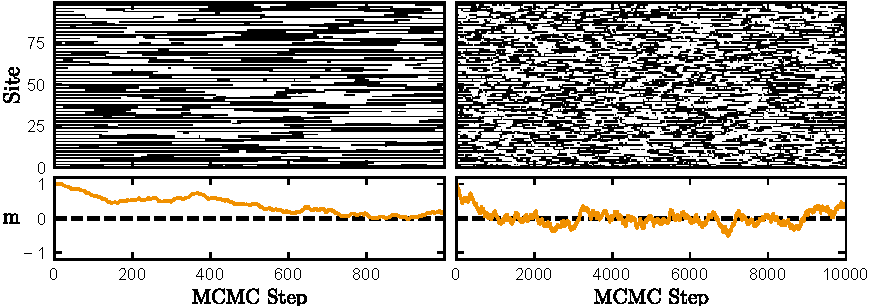
\includegraphics[width=\columnwidth]{pdf_figs/raw_steps_single_flip.pdf}
  \caption{An MCMC walk starting from the staggered charge density wave ground state for a system with $N = 100$ sites and 10,000 MCMC steps. In this simulation only a single spin can be flipped per step according to the Metropolis-Hastings Algorithm. The staggered magnetisation $m = N^{-1} \sum_i (-1)^i \; S_i$ order parameter is plotted below. At this temperature the thermal average of m is zero, while the initial state has m = 1. We see that it takes about 1000 steps for the system to converge, after which it moves about the m = 0 average with a finite auto-correlation time.  $t = 1, \alpha = 1.25, T = 3, J = U = 5 $ \label{fig:raw}}
\end{figure}

\ac{MCMC} sidesteps these issues by defining a random walk that focuses on the states with the greatest Boltzmann weight. At low temperatures this means we need only visit a few low energy states to make good estimates while at high temperatures the weights become uniform so a small number of samples distributed across the state space suffice. However we will see that the method is not without difficulties of its own.

\begin{figure}
  \centering
  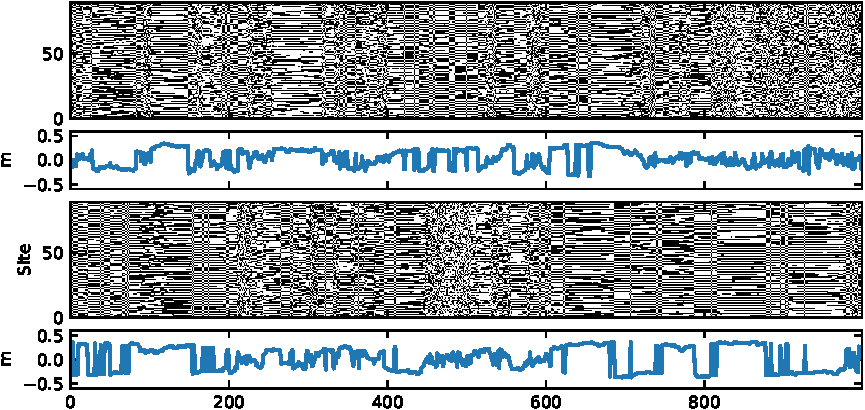
\includegraphics[width=\columnwidth]{pdf_figs/single.pdf}
  \caption{Two MCMC chains starting from the same initial state for a system with $N = 90$ sites and 1000 MCMC steps.  In this simulation the MCMC step is defined differently: an attempt is made to flip n spins, where n is drawn from Uniform(1,N). This is repeated $N^2/100$ times for each step. This trades off computation time for storage space, as it makes the samples less correlated, giving smaller statistical error for a given number of stored samples. These simulations therefore have the potential to necessitate $N^2/100$ matrix diagonalisations for every MCMC sample, though this can be cut down with caching and other tricks. $t = 1, \alpha = 1.25, T = 2.2, J = U = 5 $ \label{fig:single}}
\end{figure}

\%MCMC from an ensemble point of view In implementation \ac{MCMC} can be boiled down to choosing a transition function \$\T(\s\_\{t\} \rightarrow \s\_t+1) \$ where \(\s\) are vectors representing classical spin configurations. We start in some initial state \(\s_0\) and then repeatedly jump to new states according to the probabilities given by \(\T\). This defines a set of random walks \(\{\s_0\ldots \s_i\ldots \s_N\}\). Fig.\textasciitilde{}\ref{fig:single} shows this in practice: we have a (rather small) ensemble of \(M = 2\) walkers starting at the same point in state space and then spreading outwards by flipping spins along the way.

In pseudo-code one could write the MCMC simulation for a single walker as:

\begin{lstlisting}[language=Python]
current_state = initial_state

for i in range(N_steps):
    new_state = sample_T(current_state) 
    states[i] = current_state
\end{lstlisting}

Where the \texttt{sample\_T} function here produces a state with probability determined by the \texttt{current\_state} and the transition function \(\T\).

If we ran many such walkers in parallel we could then approximate the distribution \(p_t(\s; \s_0)\) which tells us where the walkers are likely to be after they've evolved for \(t\) steps from an initial state \(\s_0\). We need to carefully choose \(\T\) such that after a large number of steps \(k\) (the convergence time) the probability \(p_t(\s;\s_0)\) approaches the thermal distribution \(P(\s; \beta) = \Z^{-1} e^{-\beta F(\s)}\). This turns out to be quite easy to achieve using the Metropolis-Hasting algorithm.

\hypertarget{convergence-time}{%
\subsubsection{Convergence Time\}}\label{convergence-time}}

Considering \(p(\s)\) as a vector \(\vec{p}\) whose jth entry is the probability of the jth state \(p_j = p(\s_j)\), and writing \(\T\) as the matrix with entries \(T_{ij} = \T(\s_j \rightarrow \s_i)\) we can write the update rule for the ensemble probability as: \[\vec{p}_{t+1} = \T \vec{p}_t \implies \vec{p}_{t} = \T^t \vec{p}_0\] where \(\vec{p}_0\) is vector which is one on the starting state and zero everywhere else. Since all states must transition to somewhere with probability one: \(\sum_i T_{ij} = 1\).

Matrices that satisfy this are called stochastic matrices exactly because they model these kinds of Markov processes. It can be shown that they have real eigenvalues, and ordering them by magnitude, that \(\lambda_0 = 1\) and \(0 < \lambda_{i\neq0} < 1\). \%https://en.wikipedia.org/wiki/Stochastic\_matrix Assuming \(\T\) has been chosen correctly, its single eigenvector with eigenvalue 1 will be the thermal distribution \footnote{or, in the general case, any desired distribution. MCMC has found a lot of use in sampling from the complicated distributions that arise when taking a Bayesian approach to statistics.} so repeated application of the transition function eventually leads there, while memory of the initial conditions decays exponentially with a convergence time \(k\) determined by \(\lambda_1\). In practice this means that one throws away the data from the beginning of the random walk in order reduce the dependence on the initial conditions and be close enough to the target distribution.

\hypertarget{auto-correlation-time}{%
\subsubsection{Auto-correlation Time\}}\label{auto-correlation-time}}

\begin{figure}
  \centering
  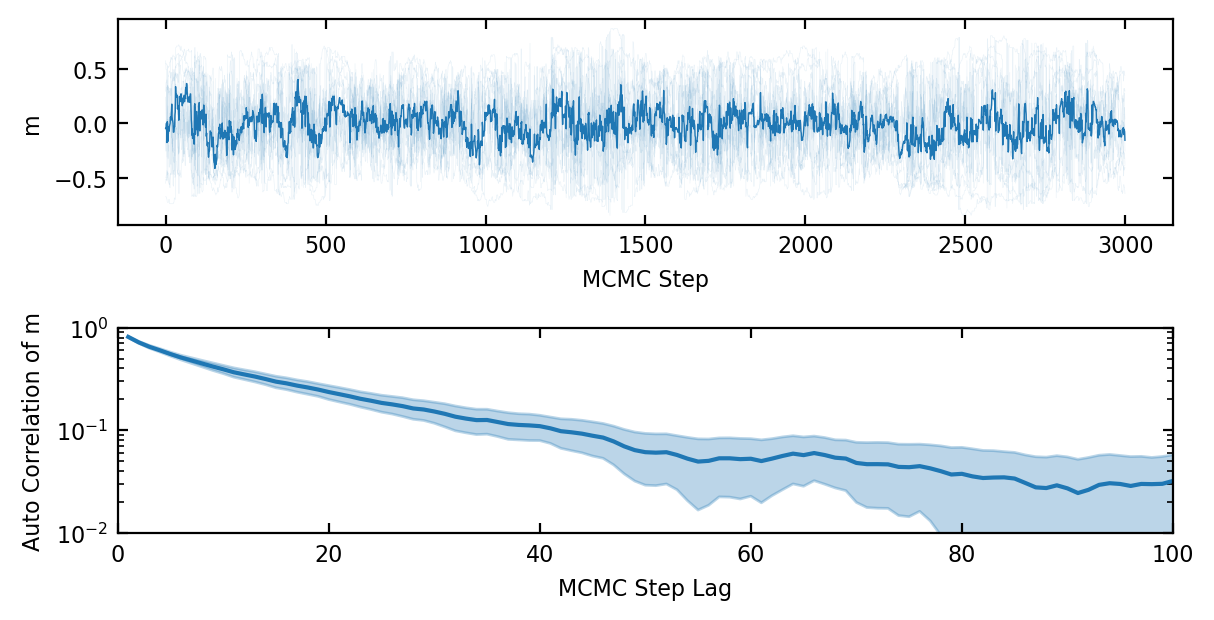
\includegraphics[width=\columnwidth]{figs/m_autocorr.png}
  \caption{(Upper) 10 MCMC chains starting from the same initial state for a system with $N = 150$ sites and 3000 MCMC steps. At each MCMC step, n spins are flipped where n is drawn from Uniform(1,N) and this is repeated $N^2/100$ times. The simulations therefore have the potential to necessitate $10*N^2$ matrix diagonalisations for each 100 MCMC steps. (Lower) The normalised auto-correlation $(\expval{m_i m_{i-j}} - \expval{m_i}\expval{m_i}) / Var(m_i))$ averaged over $i$. It can be seen that even with each MCMC step already being composed of many individual flip attempts, the auto-correlation is still non negligible and must be taken into account in the statistics. $t = 1, \alpha = 1.25, T = 2.2, J = U = 5 $ \label{fig:m_autocorr}}
\end{figure}

At this stage one might think we're done. We can indeed draw independent samples from \(P(\s; \beta)\) by starting from some arbitrary initial state and doing \(k\) steps to arrive at a sample. However a key insight is that after the convergence time, every state generated is a sample from \(P(\s; \beta)\)! They are not, however, independent samples. In Fig.\textasciitilde{}\ref{fig:raw} it is already clear that the samples of the order parameter m have some auto-correlation because only a few spins are flipped each step but even when the number of spins flipped per step is increased, Fig.\textasciitilde{}\ref{fig:m_autocorr} shows that it can be an important effect near the phase transition. Let's define the auto-correlation time \(\tau(O)\) informally as the number of MCMC samples of some observable O that are statistically equal to one independent sample.\textasciitilde{}\footnote{or equivalently as the number of MCMC steps after which the samples are correlated below some cutoff, see~@krauthIntroductionMonteCarlo1996} for a more rigorous definition involving a sum over the auto-correlation function.\} The auto-correlation time is generally shorter than the convergence time so it therefore makes sense from an efficiency standpoint to run a single walker for many MCMC steps rather than to run a huge ensemble for \(k\) steps each.

Once the random walk has been carried out for many steps, the expectation values of \(O\) can be estimated from the MCMC samples \(\s_i\): \[
    \tex{O} = \sum_{i = 0}^{N} O(\s_i) + \mathcal{O}(\frac{1}{\sqrt{N}})
\] The the samples are correlated so the N of them effectively contains less information than \(N\) independent samples would, in fact roughly \(N/\tau\) effective samples. As a consequence the variance is larger than the \(\qex{O^2} - \qex{O}^2\) form it would have if the estimates were uncorrelated. There are many methods in the literature for estimating the true variance of \(\qex{O}\) and deciding how many steps are needed but my approach has been to run a small number of parallel chains, which are independent, in order to estimate the statistical error produced. This is a slightly less computationally efficient because it requires throwing away those \(k\) steps generated before convergence multiple times but it is a conceptually simple workaround.

In summary, to do efficient simulations we want to reduce both the convergence time and the auto-correlation time as much as possible. In order to explain how, we need to introduce the Metropolis-Hasting (MH) algorithm and how it gives an explicit form for the transition function.

\hypertarget{the-metropolis-hastings-algorithm}{%
\subsubsection{The Metropolis-Hastings Algorithm\}}\label{the-metropolis-hastings-algorithm}}

MH breaks up the transition function into a proposal distribution \(q(\s \to \s')\) and an acceptance function \(\A(\s \to \s')\). \(q\) needs to be something that we can directly sample from, and in our case generally takes the form of flipping some number of spins in \(\s\), i.e if we're flipping a single random spin in the spin chain, \(q(\s \to \s')\) is the uniform distribution on states reachable by one spin flip from \(\s\). This also gives the nice symmetry property that \(q(\s \to \s') = q(\s' \to \s)\).

The proposal \(\s'\) is then accepted or rejected with an acceptance probability \(\A(\s \to \s')\), if the proposal is rejected then \(\s_{i+1} = \s_{i}\). Hence:

\[\T(x\to x') = q(x\to x')\A(x \to x')\]

When the proposal distribution is symmetric as ours is, it cancels out in the expression for the acceptance function and the Metropolis-Hastings algorithm is simply the choice: \[ \A(x \to x') = \min\left(1, e^{-\beta\;\Delta F}\right)\] Where \(F\) is the overall free energy of the system, including both the quantum and classical sector.

To implement the acceptance function in practice we pick a random number in the unit interval and accept if it is less than \(e^{-\beta\;\Delta F}\):

\begin{lstlisting}[language=Python]
current_state = initial_state

for i in range(N_steps):
    new_state = proposal(current_state)
    df = free_energy_change(current_state, new_state, parameters)

    if uniform(0,1) < exp(-beta * df):
        current_state = new_state
        
    states[i] = current_state
\end{lstlisting}

This has the effect of always accepting proposed states that are lower in energy and sometimes accepting those that are higher in energy than the current state.

\hypertarget{choosing-the-proposal-distribution}{%
\subsubsection{Choosing the proposal distribution\}}\label{choosing-the-proposal-distribution}}

\begin{figure}[H]
  \centering
  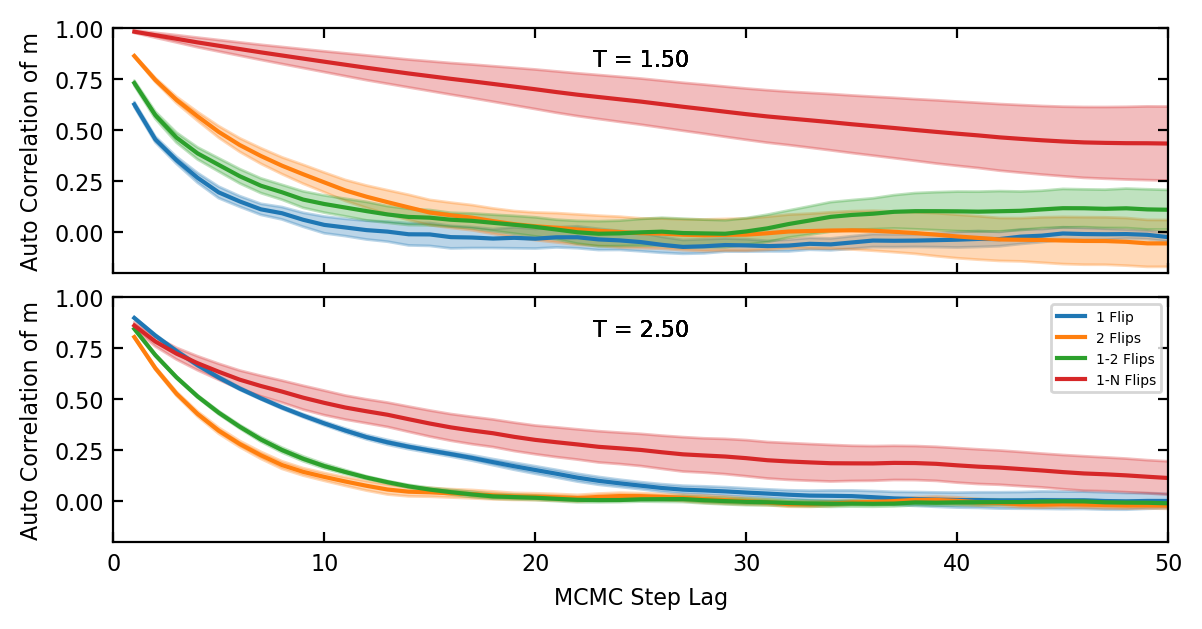
\includegraphics[width=\columnwidth]{figs/autocorr_multiple_proposals.png}
  Simulations showing how the autocorrelation of the order parameter depends on the proposal distribution used at different temperatures, we see that at $T = 1.5 < T_c$ a single spin flip is likely the best choice, while at the high temperature $T = 2.5 > T_c$ flipping two sites or a mixture of flipping two and 1 sites is likely a better choice. 
  \caption{ $t = 1, \alpha = 1.25, J = U = 5 $ \label{fig:comparison}}
\end{figure}

Now we can discuss how to minimise the auto-correlations. The general principle is that one must balance the proposal distribution between two extremes. Choose overlay small steps, like flipping only a single spin and the acceptance rate will be high because \(\Delta F\) will usually be small, but each state will be very similar to the previous and the auto-correlations will be high too, making sampling inefficient. On the other hand, overlay large steps, like randomising a large portion of the spins each step, will result in very frequent rejections, especially at low temperatures.

I evaluated a few different proposal distributions for use with the FK model.

\begin{enumerate}
\item Flipping a single random site
\item Flipping N random sites for some N
\item Choosing n from Uniform(1, N) and then flipping n sites for some fixed N.
\item Attempting to tune the proposal distribution for each parameter regime.
\end{enumerate}

Fro Figure\textasciitilde{}\ref{fig:comparison} we see that even at moderately high temperatures \(T > T_c\) flipping one or two sites is the best choice. However for some simulations at very high temperature flipping more spins is warranted. Tuning the proposal distribution automatically seems like something that would not yield enough benefit for the additional complexity it would require.

\hypertarget{two-step-trick}{%
\subsubsection{Two Step Trick}\label{two-step-trick}}

Our method already relies heavily on the split between the classical and quantum sector to derive a sign problem free MCMC algorithm but it turns out that there is a further trick we can play with it. The free energy term is the sum of an easy to compute classical energy and a more expensive quantum free energy, we can split the acceptance function into two in such as way as to avoid having to compute the full exact diagonalisation some of the time:

\begin{Shaded}
\begin{Highlighting}[]

\NormalTok{current\_state }\OperatorTok{=}\NormalTok{ initial\_state}

\ControlFlowTok{for}\NormalTok{ i }\KeywordTok{in} \BuiltInTok{range}\NormalTok{(N\_steps):}
\NormalTok{    new\_state }\OperatorTok{=}\NormalTok{ proposal(current\_state)}

\NormalTok{    df\_classical }\OperatorTok{=}\NormalTok{ classical\_free\_energy\_change(current\_state, new\_state, parameters)}
    \ControlFlowTok{if}\NormalTok{ exp(}\OperatorTok{{-}}\NormalTok{beta }\OperatorTok{*}\NormalTok{ df\_classical) }\OperatorTok{\textless{}}\NormalTok{ uniform(}\DecValTok{0}\NormalTok{,}\DecValTok{1}\NormalTok{):}
\NormalTok{        f\_quantum }\OperatorTok{=}\NormalTok{ quantum\_free\_energy(current\_state, new\_state, parameters)}
    
        \ControlFlowTok{if}\NormalTok{ exp(}\OperatorTok{{-}}\NormalTok{ beta }\OperatorTok{*}\NormalTok{ df\_quantum) }\OperatorTok{\textless{}}\NormalTok{ uniform(}\DecValTok{0}\NormalTok{,}\DecValTok{1}\NormalTok{):}
\NormalTok{          current\_state }\OperatorTok{=}\NormalTok{ new\_state}
    
\NormalTok{        states[i] }\OperatorTok{=}\NormalTok{ current\_state}
    
\end{Highlighting}
\end{Shaded}

lets cite Figure \ref{fig:binder}

lets cite to person \textcite{trebstKitaevMaterials2022}. and then multple \autocite{banerjeeProximateKitaevQuantum2016,trebstKitaevMaterials2022}. what is we surround it by spaces? \textcite{trebstKitaevMaterials2022}

\begin{figure}
\hypertarget{fig:phase_diagram}{%
\centering
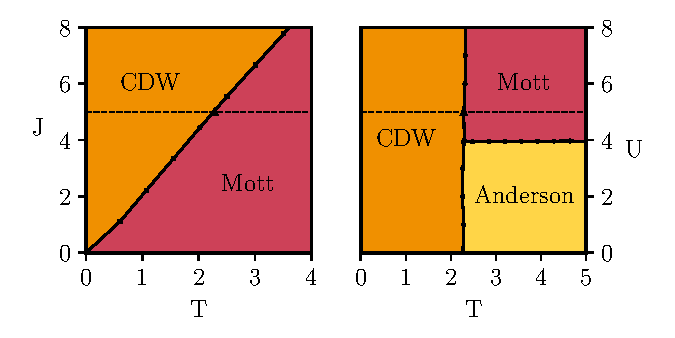
\includegraphics{pdf_figs/phase_diagram.pdf}
\caption{Phase diagrams of the long-range 1D {FK} model. (a) The TJ plane at \(U = 5\): the {CDW} ordered phase is separated from a disordered Mott insulating (MI) phase by a critical temperature \(T_c\), linear in J. (b) The TU plane at \(J = 5\): the disordered phase is split into two: at large/small U there's a MI/Anderson phase characterised by the presence/absence of a gap at \(E=0\) in the single particle energy spectrum. \(U_c\) is independent of temperature. At \(U = 0\) the fermions are decoupled from the spins forming a simple Fermi gas. (c) The order parameters, \(\tex{m^2}\)(solid) and \(1 - f\) (dashed) describing the onset of the {CDW} phase of the long-range 1D {FK} model at low temperature with staggered magnetisation \(m = N^{-1} \sum_i (-1)^i S_i\) and fermionic order parameter \(f = 2 N^{-1}\abs{\sum_i (-1)^i \; \expval{c^\dag_{i}c_{i}}}\) . (d) The crossing of the Binder cumulant, \(B = \tex{m^4} / \tex{m^2}^2\), with system size provides a diagnostic that the phase transition is not a finite size effect, it's used to estimate the critical lines shown in (a) and (b). All plots use system sizes \(N = [10,20,30,50,70,110,160,250]\) and lines are coloured from \(N = 10\) in dark blue to \(N = 250\) in yellow. The parameter values \(U = 5,\;J = 5,\;\alpha = 1.25\) except where explicitly varied.}\label{fig:phase_diagram}
}
\end{figure}

\hypertarget{introduction-1}{%
\section{Introduction}\label{introduction-1}}

The {FK} model is one of the simplest models of the correlated electron problem. It captures the essence of the interaction between itinerant and localized electrons, equivalent to a model of hopping fermions coupled to a classical Ising field. It was originally introduced to explain the metal-insulator transition in f-electron systems but in its long history it has been interpreted variously as a model of electrons and ions, binary alloys or of crystal formation~\autocite{hubbardj.ElectronCorrelationsNarrow1963,falicovSimpleModelSemiconductorMetal1969,gruberFalicovKimballModelReview1996,gruberFalicovKimballModel2006}. Despite its simplicity, the {FK} model has a rich phase diagram in \(D \geq 2\) dimensions. For example, it shows an interaction-induced gap opening even at high temperatures, similar to the corresponding Hubbard Model~\autocite{brandtThermodynamicsCorrelationFunctions1989}. In 1D, the ground state phenomenology as a function of filling can be rich~\autocite{gruberGroundStatesSpinless1990} but the system is disordered for all \(T > 0\)~\autocite{kennedyItinerantElectronModel1986}. Moreover, the model has been a test-bed for many-body methods, interest took off when an exact DMFT solution in the infinite dimensional case was found~\autocite{antipovCriticalExponentsStrongly2014,ribicNonlocalCorrelationsSpectral2016,freericksExactDynamicalMeanfield2003,herrmannNonequilibriumDynamicalCluster2016}.

The presence of the classical field makes the model amenable to an exact numerical treatment at finite temperature via a sign problem free {MCMC} algorithm~\autocite{devriesGapsDensitiesStates1993,devriesSimplifiedHubbardModel1993,antipovInteractionTunedAndersonMott2016,debskiPossibilityDetectionFinite2016,herrmannSpreadingCorrelationsFalicovKimball2018,maskaThermodynamicsTwodimensionalFalicovKimball2006}. The {MCMC} treatment motivates a view of the classical background field as a disorder potential, which suggests an intimate link to localisation physics. Indeed, thermal fluctuations of the classical sector act as disorder potentials drawn from a thermal distribution and the emergence of disorder in a translationally invariant Hamiltonian links the {FK} model to recent interest in disorder-free localisation~\autocite{smithDisorderFreeLocalization2017,smithDynamicalLocalizationMathbbZ2018,brenesManyBodyLocalizationDynamics2018}.

Dimensionality is crucial for the physics of both localisation and {FTPTs}. In 1D, disorder generally dominates, even the weakest disorder exponentially localises \emph{all} single particle eigenstates. Only longer-range correlations of the disorder potential can potentially induce delocalization~\autocite{aubryAnalyticityBreakingAnderson1980,dassarmaLocalizationMobilityEdges1990,dunlapAbsenceLocalizationRandomdimer1990}. Thermodynamically, short-range interactions cannot overcome thermal defects in 1D which prevents ordered phases at nonzero temperature~\autocite{andersonAbsenceDiffusionCertain1958,goldshteinPurePointSpectrum1977,abrahamsScalingTheoryLocalization1979,kramerLocalizationTheoryExperiment1993}. However, the absence of an {FTPT} in the short ranged {FK} chain is far from obvious because the Ruderman-Kittel-Kasuya-Yosida (RKKY) interaction mediated by the fermions~\autocite{kasuyaTheoryMetallicFerro1956,rudermanIndirectExchangeCoupling1954,vanvleckNoteInteractionsSpins1962,yosidaMagneticPropertiesCuMn1957} decays as \(r^{-1}\) in 1D~\autocite{rusinCalculationRKKYRange2017a}. This could in principle induce the necessary long-range interactions for the classical Ising background~\autocite{thoulessLongRangeOrderOneDimensional1969,peierlsIsingModelFerromagnetism1936}. However, Kennedy and Lieb established rigorously that at half-filling a {CDW} phase only exists at \(T = 0\) for the 1D {FK} model~\autocite{kennedyItinerantElectronModel1986}.

Here, we construct a generalised one-dimensional {FK} model with long-range interactions which induces the otherwise forbidden {CDW} phase at non-zero temperature. We find a rich phase diagram with a CDW FTPT and interaction-tuned Anderson versus Mott localized phases similar to the 2D {FK} model~\autocite{antipovInteractionTunedAndersonMott2016}. We explore the localization properties of the fermionic sector and find that the localisation lengths vary dramatically across the phases and for different energies. Although moderate system sizes indicate the coexistence of localized and delocalized states within the CDW phase, we find quantitatively similar behaviour in a model of uncorrelated binary disorder on a {CDW} background. For large system sizes, i.e.~for our 1D disorder model we can treat linear sizes of several thousand sites, we find that all states are eventually localized with a localization length which diverges towards zero temperature.

The paper is organised as follows. First, we introduce the model and present its phase diagram. Second, we present the methods used to solve it numerically. Last, we investigate the model's localisation properties and conclude.

\hypertarget{the-long-ranged-falikov-kimball-model}{%
\section{The Long-Ranged Falikov-Kimball Model}\label{the-long-ranged-falikov-kimball-model}}

We interpret the {FK} model as a model of spinless fermions, \(c^\dag_{i}\), hopping on a 1D lattice against a classical Ising spin background, \(S_i \in {\pm \frac{1}{2}}\). The fermions couple to the spins via an onsite interaction with strength \(U\) which we supplement by a long-range interaction, \(J_{ij} = 4\kappa J (-1)^{\abs{i-j}} \abs{i-j}^{-\alpha}\), between the spins. The normalisation, \(\kappa^{-1} = \sum_{i=1}^{N} i^{-\alpha}\), renders the 0th order mean field critical temperature independent of system size. The hopping strength of the electrons, \(t = 1\), sets the overall energy scale and we concentrate throughout on the particle-hole symmetric point at zero chemical potential and half filling~\autocite{gruberFalicovKimballModelReview1996}. ~ \[\begin{aligned}
H_{\mathrm{FK}} = & \;U \sum_{i} S_i\;(c^\dag_{i}c_{i} - \tfrac{1}{2}) -\;t \sum_{i} (c^\dag_{i}c_{i+1} + \textit{h.c.)}\\ 
 &  + \sum_{i, j}^{N} J_{ij}  S_i S_j \nonumber
\label{eq:HFK}\end{aligned}\]

In two or more dimensions, the \(J\!=0\!\) {FK} model has a {FTPT} to the {CDW} phase with non-zero staggered magnetisation \(m = N^{-1} \sum_i (-1)^i \; S_i\) and fermionic order parameter \(f = 2 N^{-1}\abs{\sum_i (-1)^i \; \expval{c^\dag_{i}c_{i}}}\)~\autocite{antipovInteractionTunedAndersonMott2016,maskaThermodynamicsTwodimensionalFalicovKimball2006}. This only exists at zero temperature in the short ranged 1D model~\autocite{kennedyItinerantElectronModel1986}. To study the {CDW} phase at finite temperature in 1D, we add an additional coupling that is both long-ranged and staggered by a factor \((-1)^{|i-j|}\). The additional coupling stabilises the Antiferromagnetic (AFM) order of the Ising spins which promotes the finite temperature {CDW} phase of the fermionic sector.

Taking the limit \(U = 0\) decouples the spins from the fermions, which gives a spin sector governed by a classical {LRI} model. Note, the transformation of the spins \(S_i \to (-1)^{i} S_i\) maps the AFM model to the FM one. We recall that Peierls' classic argument can be extended to show that, for the 1D {LRI} model, a power law decay of \(\alpha < 2\) is required for a {FTPT} as the energy of defect domain then scales with the system size and can overcome the entropic contribution. A renormalisation group analysis supports this finding and shows that the critical exponents are only universal for \(\alpha \leq 3/2\)~\autocite{ruelleStatisticalMechanicsOnedimensional1968,thoulessLongRangeOrderOneDimensional1969,angeliniRelationsShortrangeLongrange2014}. In the following, we choose \(\alpha = 5/4\) to avoid this additional complexity.

To improve the scaling of finite size effects, we make the replacement \(\abs{i - j}^{-\alpha} \rightarrow \abs{f(i - j)}^{-\alpha}\), in both \(J_{ij}\) and \(\kappa\), where \(f(x) = \frac{N}{\pi}\sin \frac{\pi x}{N}\), which is smooth across the circular boundary~\autocite{fukuiOrderNClusterMonte2009}. We only consider even system sizes given that odd system sizes are not commensurate with a {CDW} state.

\hypertarget{the-phase-diagram}{%
\section{The Phase Diagram}\label{the-phase-diagram}}

Figs.~{[}\protect\hyperlink{fig:phase_diagram}{1}a{]} and {[}\protect\hyperlink{fig:phase_diagram}{1}b{]} show the phase diagram for constant \(U=5\) and constant \(J=5\), respectively. We determined the transition temperatures from the crossings of the Binder cumulants \(B_4 = \tex{m^4}/\tex{m^2}^2\)~\autocite{binderFiniteSizeScaling1981}. For a representative set of parameters, Fig.~{[}\protect\hyperlink{fig:phase_diagram}{1}c{]} shows the order parameter \(\tex{m}^2\). Fig.~{[}\protect\hyperlink{fig:phase_diagram}{1}d{]} shows the Binder cumulants, both as functions of system size and temperature. The crossings confirm that the system has a {FTPT} and that the ordered phase is not a finite size effect.

The CDW transition temperature is largely independent from the strength of the interaction \(U\). This demonstrates that the phase transition is driven by the long-range term \(J\) with little effect from the coupling to the fermions \(U\). The physics of the spin sector in our long-range {FK} model mimics that of the {LRI} model and is not significantly altered by the presence of the fermions, which shows that the long range tail expected from a basic fermion mediated RKKY interaction between the Ising spins is absent.

Our main interest concerns the additional structure of the fermionic sector in the high temperature phase. Following Ref.~\autocite{antipovInteractionTunedAndersonMott2016}, we can distinguish between the Mott and Anderson insulating phases. The former is characterised by a gapped {DOS} in the absence of a {CDW}. Thus, the opening of a gap for large \(U\) is distinct from the gap-opening induced by the translational symmetry breaking in the CDW state below \(T_c\), see also Fig.~{[}\protect\hyperlink{fig:band_opening}{3}a{]}. The Anderson phase is gapless but, as we explain below, shows localised fermionic eigenstates.

\hypertarget{markov-chain-monte-carlo-and-emergent-disorder}{%
\section{Markov Chain Monte Carlo and Emergent Disorder}\label{markov-chain-monte-carlo-and-emergent-disorder}}

The results for the phase diagram were obtained with a classical {MCMC} method which we discuss in the following. It allows us to solve our long-range {FK} model efficiently, yielding unbiased estimates of thermal expectation values and linking it to disorder physics in a translationally invariant setting.

Since the spin configurations are classical, the Hamiltonian can be split into a classical spin part \(H_s\) and an operator valued part \(H_c\). \[\begin{aligned}
H_s& = - \frac{U}{2}S_i + \sum_{i, j}^{N} J_{ij} S_i S_j \\
H_c& = \sum_i U S_i c^\dag_{i}c_{i} -t(c^\dag_{i}c_{i+1} + c^\dag_{i+1}c_{i}) \end{aligned}\] The partition function can then be written as a sum over spin configurations, \(\vec{S} = (S_0, S_1...S_{N-1})\): \[\begin{aligned}
\Z = \Tr e^{-\beta H}= \sum_{\vec{S}} e^{-\beta H_s} \Tr_c e^{-\beta H_c} .\end{aligned}\] The contribution of \(H_c\) to the grand canonical partition function can be obtained by performing the sum over eigenstate occupation numbers giving \(-\beta F_c[\vec{S}] = \sum_k \ln{(1 + e^{- \beta \epsilon_k})}\) where \({\epsilon_k[\vec{S}]}\) are the eigenvalues of the matrix representation of \(H_c\) determined through exact diagonalisation. This gives a partition function containing a classical energy which corresponds to the long-range interaction of the spins, and a free energy which corresponds to the quantum subsystem. \[\begin{aligned}
\Z = \sum_{\vec{S}} e^{-\beta H_S[\vec{S}] - \beta F_c[\vec{S}]} = \sum_{\vec{S}} e^{-\beta E[\vec{S}]}\end{aligned}\]

{MCMC} defines a weighted random walk over the spin states \((\vec{S}_0, \vec{S}_1, \vec{S}_2, ...)\), such that the likelihood of visiting a particular state converges to its Boltzmann probability \(p(\vec{S}) = \Z^{-1} e^{-\beta E}\)~\autocite{binderGuidePracticalWork1988,kerteszAdvancesComputerSimulation1998,wolffMonteCarloErrors2004}. Hence, any observable can be estimated as a mean over the states visited by the walk. \[\begin{aligned}
 \label{eq:thermal_expectation}
\tex{O}& = \sum_{\vec{S}} p(\vec{S}) \tex{O}_{\vec{S}} = \sum_{i = 0}^{M} \tex{O}_{\vec{S}_i} + \mathcal{O}(\tfrac{1}{\sqrt{M}})\\
\tex{O}_{\vec{S}}& = \sum_{\nu} n_F(\epsilon_{\nu}) \expval{O}{\nu}\end{aligned}\] Where \(\nu\) runs over the eigenstates of \(H_c\) for a particular spin configuration and \(n_F(\epsilon) = \left(e^{-\beta\epsilon} + 1\right)^{-1}\) is the Fermi function.

The choice of the transition function for {MCMC} is under-determined as one only needs to satisfy a set of balance conditions for which there are many solutions~\autocite{kellyReversibilityStochasticNetworks1981}. Here, we incorporate a modification to the standard Metropolis-Hastings algorithm~\autocite{hastingsMonteCarloSampling1970} gleaned from Krauth~\autocite{krauthIntroductionMonteCarlo1998}. Let us first recall the standard algorithm which decomposes the transition probability into \(\T(a \to b) = \p(a \to b)\A(a \to b)\). Here, \(\p\) is the proposal distribution that we can directly sample from while \(\A\) is the acceptance probability. The standard Metropolis-Hastings choice is \[\A(a \to b) = \min\left(1, \frac{\p(b\to a)}{\p(a\to b)} e^{-\beta \Delta E}\right)\;,\] with \(\Delta E = E_b - E_a\). The walk then proceeds by sampling a state \(b\) from \(\p\) and moving to \(b\) with probability \(\A(a \to b)\). The latter operation is typically implemented by performing a transition if a uniform random sample from the unit interval is less than \(\A(a \to b)\) and otherwise repeating the current state as the next step in the random walk. The proposal distribution is often symmetric so does not appear in \(\A\). Here, we flip a small number of sites in \(b\) at random to generate proposals, which is indeed symmetric.

In our computations~\autocite{hodsonMCMCFKModel2021} we employ a modification of the algorithm which is based on the observation that the free energy of the {FK} system is composed of a classical part which is much quicker to compute than the quantum part. Hence, we can obtain a computational speedup by first considering the value of the classical energy difference \(\Delta H_s\) and rejecting the transition if the former is too high. We only compute the quantum energy difference \(\Delta F_c\) if the transition is accepted. We then perform a second rejection sampling step based upon it. This corresponds to two nested comparisons with the majority of the work only occurring if the first test passes and has the acceptance function \[\A(a \to b) = \min\left(1, e^{-\beta \Delta H_s}\right)\min\left(1, e^{-\beta \Delta F_c}\right)\;.\]

See Appendix~\protect\hyperlink{app:balance}{{[}app:balance{]}} for a proof that this satisfies the detailed balance condition.

For the model parameters used in Fig.~\protect\hyperlink{fig:indiv_IPR}{2}, we find that with our new scheme the matrix diagonalisation is skipped around 30\% of the time at \(T = 2.5\) and up to 80\% at \(T = 1.5\). We observe that for \(N = 50\), the matrix diagonalisation, if it occurs, occupies around 60\% of the total computation time for a single step. This rises to 90\% at N = 300 and further increases for larger N. We therefore get the greatest speedup for large system sizes at low temperature where many prospective transitions are rejected at the classical stage and the matrix computation takes up the greatest fraction of the total computation time. The upshot is that we find a speedup of up to a factor of 10 at the cost of very little extra algorithmic complexity.

Our two-step method should be distinguished from the more common method for speeding up {MCMC} which is to add asymmetry to the proposal distribution to make it as similar as possible to \(\min\left(1, e^{-\beta \Delta E}\right)\). This reduces the number of rejected states, which brings the algorithm closer in efficiency to a direct sampling method. However it comes at the expense of requiring a way to directly sample from this complex distribution, a problem which {MCMC} was employed to solve in the first place. For example, recent work trains restricted Boltzmann machines (RBMs) to generate samples for the proposal distribution of the {FK} model~\autocite{huangAcceleratedMonteCarlo2017}. The RBMs are chosen as a parametrisation of the proposal distribution that can be efficiently sampled from while offering sufficient flexibility that they can be adjusted to match the target distribution. Our proposed method is considerably simpler and does not require training while still reaping some of the benefits of reduced computation.

\hypertarget{localisation-properties}{%
\section{Localisation Properties}\label{localisation-properties}}

The {MCMC} formulation suggests viewing the spin configurations as a form of annealed binary disorder whose probability distribution is given by the Boltzmann weight \(e^{-\beta H_S[\vec{S}] - \beta F_c[\vec{S}]}\). This makes apparent the link to the study of disordered systems and Anderson localisation. While these systems are typically studied by defining the probability distribution for the quenched disorder potential externally, here we have a translation invariant system with disorder as a natural consequence of the Ising background field conserved under the dynamics.

In the limits of zero and infinite temperature, our model becomes a simple tight-binding model for the fermions. At zero temperature, the spin background is in one of the two translation invariant AFM ground states with two gapped fermionic CDW bands at energies \[E_{\pm} = \pm\sqrt{\frac{1}{4}U^2 + 2t^2(1 + \cos ka)^2}\;.\]

At infinite temperature, all the spin configurations become equally likely and the fermionic model reduces to one of binary uncorrelated disorder in which all eigenstates are Anderson localised~\autocite{abrahamsScalingTheoryLocalization1979}. An Anderson localised state centered around \(r_0\) has magnitude that drops exponentially over some localisation length \(\xi\) i.e \(|\psi(r)|^2 \sim \exp{-\abs{r - r_0}/\xi}\). Calculating \(\xi\) directly is numerically demanding. Therefore, we determine if a given state is localised via the energy-resolved {IPR} and the {DOS} defined as \[\begin{aligned}
\mathrm{DOS}(\vec{S}, \omega)& = N^{-1} \sum_{i} \delta(\epsilon_i - \omega)\\
\mathrm{IPR}(\vec{S}, \omega)& = \; N^{-1} \mathrm{DOS}(\vec{S}, \omega)^{-1} \sum_{i,j} \delta(\epsilon_i - \omega)\;\psi^{4}_{i,j}\end{aligned}\] where \(\epsilon_i\) and \(\psi_{i,j}\) are the \(i\)th energy level and \(j\)th element of the corresponding eigenfunction, both dependent on the background spin configuration \(\vec{S}\).

The scaling of the IPR with system size \[\mathrm{IPR} \propto N^{-\tau}\] depends on the localisation properties of states at that energy. For delocalised states, e.g.~Bloch waves, \(\tau\) is the physical dimension. For fully localised states \(\tau\) goes to zero in the thermodynamic limit. However, for special types of disorder such as binary disorder, the localisation lengths can be large comparable to the system size at hand, which can make it difficult to extract the correct scaling. An additional complication arises from the fact that the scaling exponent may display intermediate behaviours for correlated disorder and in the vicinity of a localisation-delocalisation transition~\autocite{kramerLocalizationTheoryExperiment1993,eversAndersonTransitions2008a}. The thermal defects of the CDW phase lead to a binary disorder potential with a finite correlation length, which in principle could result in delocalized eigenstates.

The key question for our system is then: How is the \(T=0\) CDW phase with fully delocalized fermionic states connected to the fully localized phase at high temperatures?

\begin{figure}
\hypertarget{fig:indiv_IPR}{%
\centering
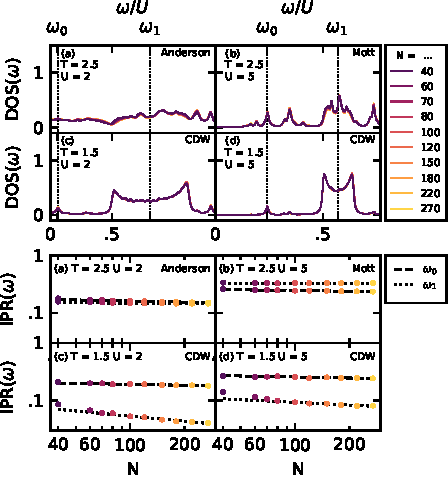
\includegraphics{pdf_figs/indiv_IPR.pdf}
\caption{Energy resolved DOS(\(\omega\)) and \(\tau\) (the scaling exponent of IPR(\(\omega\)) against system size \(N\)). The left column shows the Anderson phase \(U = 2\) at high \(T = 2.5\) and the CDW phase at low \(T = 1.5\) temperature. IPRs are evaluated for one of the in-gap states \(\omega_0/U = 0.057\) and the center of the band \(\omega_1\) \(U = 0.81\). The right column shows instead the Mott and CDW phases at \(U = 5\) with \(\omega_0/U = 0.24\) and \(\omega_1/U = 0.571\). For all the plots \(J = 5,\;\alpha = 1.25\) and the fits for \(\tau\) use system sizes greater than 60. The measured \(\tau_0,\tau_1\) for each figure are: (a) \((0.06\pm0.01, 0.02\pm0.01\) (b) \(0.04\pm0.02, 0.00\pm0.01\) (c) \(0.05\pm0.03, 0.30\pm0.03\) (d) \(0.06\pm0.04, 0.15\pm0.05\) We show later that the apparent scaling of the IPR with system size can be explained by the changing defect density with system size rather than due to delocalisation of the states.}\label{fig:indiv_IPR}
}
\end{figure}

\begin{figure}
\hypertarget{fig:band_opening}{%
\centering
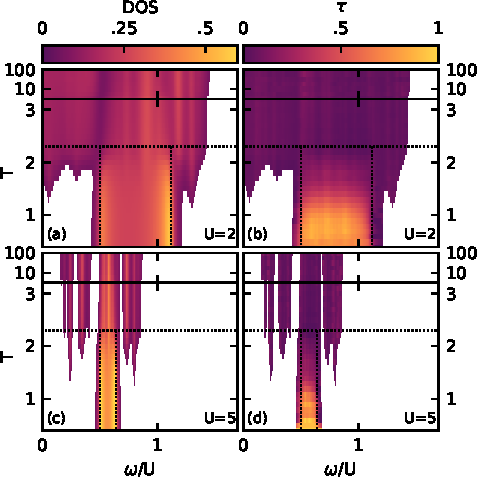
\includegraphics{pdf_figs/gap_openingboth.pdf}
\caption{The {DOS} (a and c) and scaling exponent \(\tau\) (b and d) as a function of energy and temperature. (a) and (b) show the system transitioning from the CDW phase to the gapless Anderson insulating one at \(U=2\) while (c) and (d) show the CDW to gapped Mott phase transition at \(U=5\). Regions where the DOS is close to zero are shown a white. The scaling exponent \(\tau\) is obtained from fits to \(IPR(N) = A N^{-\lambda}\) for a range of system sizes. \(U = 5,\;J = 5,\;\alpha = 1.25\)}\label{fig:band_opening}
}
\end{figure}

\begin{figure}
\hypertarget{fig:indiv_IPR_disorder}{%
\centering
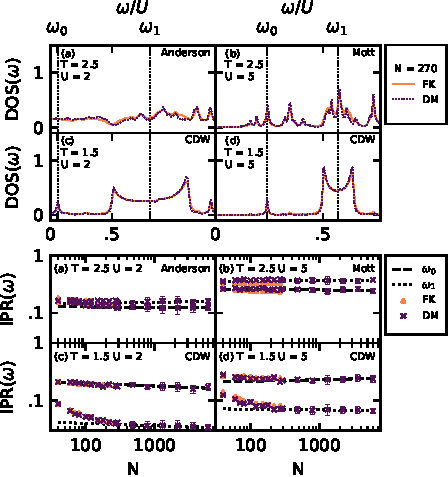
\includegraphics{pdf_figs/indiv_IPR_disorder.pdf}
\caption{A comparison of the full {FK} model to a simple binary disorder model (DM) with a CDW wave background perturbed by uncorrelated defects at density \(0 < \rho < 1\) matched to the largest corresponding FK model. As in Fig~\protect\hyperlink{fig:indiv_IPR}{2}, the Energy resolved DOS(\(\omega\)) and \(\tau\) are shown. The DOSs match well and this data makes clear that the apparent scaling of IPR with system size is a finite size effect due to weak localisation~\autocite{antipovInteractionTunedAndersonMott2016}, hence all the states are indeed localised as one would expect in 1D. The disorder model \(\tau_0,\tau_1\) for each figure are: (a) \(0.01\pm0.05, -0.02\pm0.06\) (b) \(0.01\pm0.04, -0.01\pm0.04\) (c) \(0.05\pm0.06, 0.04\pm0.06\) (d) \(-0.03\pm0.06, 0.01\pm0.06\). The lines are fit on system sizes \(N > 400\)}\label{fig:indiv_IPR_disorder}
}
\end{figure}

Fig.~\protect\hyperlink{fig:indiv_IPR}{2} shows the {DOS} and \(\tau\), the scaling exponent of the IPR with system size, for a representative set of parameters covering all three phases. The DOS is symmetric about \(0\) because of the particle hole symmetry of the model. At high temperatures, all of the eigenstates are localised in both the Mott and Anderson phases (with \(\tau \leq 0.07\) for our system sizes). We also checked that the states are localised by direct inspection. Note that there are in-gap states for instance at \(\omega_0\), below the upper band which are localized and smoothly connected across the phase transition.

In the CDW phases at \(U=2\) and \(U=5\), we find for the states within the gapped CDW bands, e.g.~at \(\omega_1\), scaling exponents \(\tau = 0.30\pm0.03\) and \(\tau = 0.15\pm0.05\), respectively. This surprising finding suggests that the CDW bands are partially delocalised with multi-fractal behaviour of the wavefunctions~\autocite{eversAndersonTransitions2008a}. This phenomenon would be unexpected in a 1D model as they generally do not support delocalisation in the presence of disorder except as the result of correlations in the emergent disorder potential~\autocite{croyAndersonLocalization1D2011,goldshteinPurePointSpectrum1977}. However, we later show by comparison to an uncorrelated Anderson model that these nonzero exponents are a finite size effect and the states are localised with a finite \(\xi\) similar to the system size. As a result, the IPR does not scale correctly until the system size has grown much larger than \(\xi\). Fig.~{[}\protect\hyperlink{fig:indiv_IPR_disorder}{4}{]} shows that the scaling of the IPR in the CDW phase does flatten out eventually.

Next, we use the {DOS} and the scaling exponent \(\tau\) to explore the localisation properties over the energy-temperature plane in Fig.~\protect\hyperlink{fig:band_opening}{3}. Gapped areas are shown in white, which highlights the distinction between the gapped Mott phase and the ungapped Anderson phase. In-gap states appear just below the critical point, smoothly filling the bandgap in the Anderson phase and forming islands in the Mott phase. As in the finite~\autocite{zondaGaplessRegimeCharge2019} and infinite dimensional~\autocite{hassanSpectralPropertiesChargedensitywave2007} cases, the in-gap states merge and are pushed to lower energy for decreasing U as the \(T=0\) CDW gap closes. Intuitively, the presence of in-gap states can be understood as a result of domain wall fluctuations away from the AFM ordered background. These domain walls act as local potentials for impurity-like bound states~\autocite{zondaGaplessRegimeCharge2019}.

In order to understand the localization properties we can compare the behaviour of our model with that of a simpler Anderson disorder model (DM) in which the spins are replaced by a {CDW} background with uncorrelated binary defect potentials, see Appendix~\protect\hyperlink{app:disorder_model}{{[}app:disorder\_model{]}}. Fig.~{[}\protect\hyperlink{fig:indiv_IPR_disorder}{4}{]} compares the FK model to the disorder model at different system sizes, matching the defect densities of the disorder model to the FK model at \(N = 270\) above and below the CDW transition. We find very good, even quantitative, agreement between the FK and disorder models, which suggests that correlations in the spin sector do not play a significant role. As we can sample directly from the disorder model, rather than through MCMC, the samples are uncorrelated. Hence we can evaluate much larger system sizes with the disorder model which enables us to pin down the correct localisation effects. In particular, what appear to be delocalized states for small system sizes eventually turn out to be states with large localization length. The localization length diverges towards the ordered zero temperature CDW state. Overall, we see that the interplay of interactions, here manifest as a peculiar binary potential, and localization can be very intricate and the added advantage of our 1D model is that we can explore very large system sizes for a complete understanding.

\hypertarget{discussion-conclusion}{%
\section{Discussion \& Conclusion}\label{discussion-conclusion}}

The {FK} model is one of the simplest non-trivial models of interacting fermions. We studied its thermodynamic and localisation properties brought down in dimensionality to 1D by adding a novel long-ranged coupling designed to stabilise the {CDW} phase present in dimension two and above. Our hybrid {MCMC} approach elucidates a disorder-free localization mechanism within our translationally invariant system. Further, we demonstrate a significant speedup over the naive method. We show that our long-range {FK} in 1D retains much of the rich phase diagram of its higher dimensional cousins. Careful scaling analysis indicates that all the single particle eigenstates eventually localise at nonzero temperature albeit only for very large system sizes of several thousand.

Our work raises a number of interesting questions for future research. A straightforward but numerically challenging problem is to pin down the model's behaviour closer to the critical point where correlations in the spin sector would become significant. Would this modify the localisation behaviour? Similar to other soluble models of disorder-free localisation, we expect intriguing out-of equilibrium physics, for example slow entanglement dynamics akin to more generic interacting systems~\autocite{hartLogarithmicEntanglementGrowth2020}. One could also investigate whether the rich ground state phenomenology of the FK model as a function of filling~\autocite{gruberGroundStatesSpinless1990} such as the devil's staircase~\autocite{michelettiCompleteDevilTextquotesingles1997} could be stabilised at finite temperature. In a broader context, we envisage that long-range interactions can also be used to gain a deeper understanding of the temperature evolution of topological phases. One example would be a long-ranged {FK} version of the celebrated Su-Schrieffer-Heeger model where one could explore the interplay of topological bound states and thermal domain wall defects. Finally, the rich physics of our model should be realizable in systems with long-range interactions, such as trapped ion quantum simulators, where one can also explore the fully interacting regime with a dynamical background field.

\hypertarget{acknowledgments}{%
\section{Acknowledgments}\label{acknowledgments}}

We wish to acknowledge the support of Alexander Belcik who was involved with the initial stages of the project. We thank Angus MacKinnon for helpful discussions, Sophie Nadel for input when preparing the figures and acknowledge support from the Imperial-TUM flagship partnership. This work was supported in part by the Engineering and Physical Sciences Research Council (EPSRC) \href{https://gtr.ukri.org/project/145404DD-ABAD-4CFB-A2D8-152A6AFCCEB7\#/tabOverview}{Project No.~2120140}.

\hypertarget{detailed-balance}{%
\section[ DETAILED BALANCE]{\texorpdfstring{\protect\hypertarget{app:balance}{}{} DETAILED BALANCE}{ DETAILED BALANCE}}\label{detailed-balance}}

Given a {MCMC} algorithm with target distribution \(\pi(a)\) and transition function \(\T\) the detailed balance condition is sufficient (along with some technical constraints \autocite{wolffMonteCarloErrors2004}) to guarantee that in the long time limit the algorithm produces samples from \(\pi\). \[\pi(a)\T(a \to b) = \pi(b)\T(b \to a)\]

In pseudo-code, our two step method corresponds to two nested comparisons with the majority of the work only occurring if the first test passes:

\begin{Shaded}
\begin{Highlighting}[]
\NormalTok{current\_state }\OperatorTok{=}\NormalTok{ initial\_state}

\ControlFlowTok{for}\NormalTok{ i }\KeywordTok{in} \BuiltInTok{range}\NormalTok{(N\_steps):}
\NormalTok{  new\_state }\OperatorTok{=}\NormalTok{ proposal(current\_state)}

\NormalTok{  c\_dE }\OperatorTok{=}\NormalTok{ classical\_energy\_change(}
\NormalTok{                               current\_state,}
\NormalTok{                               new\_state)}
  \ControlFlowTok{if}\NormalTok{ uniform(}\DecValTok{0}\NormalTok{,}\DecValTok{1}\NormalTok{) }\OperatorTok{\textless{}}\NormalTok{ exp(}\OperatorTok{{-}}\NormalTok{beta }\OperatorTok{*}\NormalTok{ c\_dE):}
\NormalTok{    q\_dF }\OperatorTok{=}\NormalTok{ quantum\_free\_energy\_change(}
\NormalTok{                                current\_state,}
\NormalTok{                                new\_state)}
    \ControlFlowTok{if}\NormalTok{ uniform(}\DecValTok{0}\NormalTok{,}\DecValTok{1}\NormalTok{) }\OperatorTok{\textless{}}\NormalTok{ exp(}\OperatorTok{{-}}\NormalTok{ beta }\OperatorTok{*}\NormalTok{ q\_dF):}
\NormalTok{      current\_state }\OperatorTok{=}\NormalTok{ new\_state}

\NormalTok{    states[i] }\OperatorTok{=}\NormalTok{ current\_state}
\end{Highlighting}
\end{Shaded}

Defining \(r_c = e^{-\beta H_c}\) and \(r_q = e^{-\beta F_q}\) our target distribution is \(\pi(a) = r_c r_q\). This method has \(\T(a\to b) = q(a\to b)\A(a \to b)\) with symmetric \(p(a \to b) = \p(b \to a)\) and \(\A = \min\left(1, r_c\right) \min\left(1, r_q\right)\)

Substituting this into the detailed balance equation gives: \[\T(a \to b)/\T(b \to a) = \pi(b)/\pi(a) = r_c r_q\]

Taking the LHS and substituting in our transition function: \[\begin{aligned}
\T(a \to b)/\T(b \to a) = \frac{\min\left(1, r_c\right) \min\left(1, r_q\right)}{ \min\left(1, 1/r_c\right) \min\left(1, 1/r_q\right)}\end{aligned}\]

which simplifies to \(r_c r_q\) as \(\min(1,r)/\min(1,1/r) = r\) for \(r > 0\).

\hypertarget{uncorrelated-disorder-model}{%
\section[ UNCORRELATED DISORDER MODEL]{\texorpdfstring{\protect\hypertarget{app:disorder_model}{}{} UNCORRELATED DISORDER MODEL}{ UNCORRELATED DISORDER MODEL}}\label{uncorrelated-disorder-model}}

The disorder model referred to in the main text is defined by replacing the spin degree of freedom in the FK model \(S_i = \pm \tfrac{1}{2}\) with a disorder potential \(d_i = \pm \tfrac{1}{2}\) controlled by a defect density \(\rho\) such that \(d_i = -\tfrac{1}{2}\) with probability \(\rho/2\) and \(d_i = \tfrac{1}{2}\) otherwise. \(\rho/2\) is used rather than \(\rho\) so that the disorder potential takes on the zero temperature CDW ground state at \(\rho = 0\) and becomes a random choice over spin states at \(\rho = 1\) i.e the infinite temperature limit. ~ \[\begin{aligned}
H_{\mathrm{DM}} = & \;U \sum_{i} (-1)^i \; d_i \;(c^\dag_{i}c_{i} - \tfrac{1}{2}) \\
& -\;t \sum_{i} c^\dag_{i}c_{i+1} + c^\dag_{i+1}c_{i} \nonumber\end{aligned}\]

\begin{Shaded}
\begin{Highlighting}[]

\end{Highlighting}
\end{Shaded}
